\documentclass{presentation}
\newcommand{\wbf}{\mathbf{w}}
\newcommand{\Wbf}{\mathbf{W}}
\newcommand{\xbf}{\ensuremath{\mathbf{x}}}
\newcommand{\zbf}{\ensuremath{\mathbf{z}}}
\newcommand{\zerobf}{\mathbf{0}}
\newcommand{\h}{h}
\newcommand{\dist}{\mathrm{dist}}

\newcommand{\Acal}{\ensuremath{\mathcal{A}}}
\newcommand{\Bcal}{\ensuremath{\mathcal{B}}}
\newcommand{\Ccal}{\ensuremath{\mathcal{C}}}
\newcommand{\Dcal}{\ensuremath{\mathcal{D}}}
\newcommand{\Fcal}{\ensuremath{\mathcal{F}}}
\newcommand{\Hcal}{\ensuremath{\mathcal{H}}}
\newcommand{\Mcal}{\ensuremath{\mathcal{M}}}
\newcommand{\Ncal}{\ensuremath{\mathcal{N}}}
\newcommand{\Pcal}{\ensuremath{\mathcal{P}}}
\newcommand{\Scal}{\ensuremath{\mathcal{S}}}
\newcommand{\Tcal}{\ensuremath{\mathcal{T}}}
\newcommand{\Xcal}{\ensuremath{\mathcal{X}}}
\newcommand{\Ycal}{\ensuremath{\mathcal{Y}}}
\newcommand{\Zcal}{\ensuremath{\mathcal{Z}}}

\newcommand{\Ebb}{\ensuremath{\mathbb{E}}}
\newcommand{\Pbb}{\ensuremath{\mathbb{P}}}
\newcommand{\Rbb}{\ensuremath{\mathbb{R}}}
\newcommand{\Nbb}{\ensuremath{\mathbb{N}}}

\newcommand{\Rfrak}{\ensuremath{\mathfrak{R}}}

\newcommand{\RA}{\right\rangle}
\newcommand{\LA}{\left\langle}
\newcommand{\LB}{\left[}
\newcommand{\RB}{\right]}
\newcommand{\LC}{\left\{}
\newcommand{\LM}{\left\|}
\newcommand{\RM}{\right\|}
%\newcommand{\RC}{\right\}}
%\newcommand{\RN}{\right\vert}
\newcommand{\LN}{\left\vert}
\newcommand{\LP}{\left(}
\newcommand{\RP}{\right)}

\newcommand{\wrt}{{\it w.r.t.}\xspace}
\newcommand{\eg}{{\it e.g.}\xspace}
\newcommand{\ie}{{\it i.e.}\xspace}
\newcommand{\iid}{{\it i.i.d.}\xspace}

\newcommand{\defeq}{:=}

\DeclareMathOperator*{\EE}{\Ebb}
\DeclareMathOperator*{\PP}{\Pbb}
\DeclareMathOperator*{\argmin}{\mathrm{argmin}}
\DeclareMathOperator*{\vect}{\mathrm{vec}}
\DeclareMathOperator*{\leaky}{\mathrm{Leaky}}
\DeclareMathOperator*{\proj}{\mathrm{Proj}}

\newcommand{\Irm}{\mathrm{I}}
\newcommand{\KL}{\mathrm{KL}}
\newcommand{\KLr}{\overline{\KL}}
\newcommand{\Hell}{H^2}
\newcommand{\TV}{TV}
\newcommand{\kl}{\mathrm{kl}}
\newcommand{\W}{\mathrm{W}}
\newcommand{\Lip}{\mathrm{Lip}}

\newcommand{\D}{\Dcal}
\newcommand{\Dm}{\Dcal_{m}}
\renewcommand{\H}{\Hcal}
\newcommand{\Hb}{\overline{\Hcal}}
\newcommand{\loss}{\ell}
\renewcommand{\P}{\mathrm{P}}
\newcommand{\Q}{\mathrm{Q}}
\newcommand{\R}{\Rbb}
\newcommand{\N}{\Nbb}
\renewcommand{\S}{\Scal}
\newcommand{\Sm}{\S_m}
\newcommand{\Risk}{\text{R}}
\newcommand{\Riskhat}{\hat{\Risk}}
\newcommand{\X}{\Xcal}
\newcommand{\x}{\xbf}
\newcommand{\y}{y}
\newcommand{\Y}{\Ycal}
\newcommand{\Z}{\Zcal}
\newcommand{\z}{\zbf}
\newcommand{\varepsilonbf}{\boldsymbol{\varepsilon}}
\newcommand{\rad}{\mathdbcal{E}}
\newcommand{\DS}{\D_\S}
\newcommand{\yeast}{{\sc Yeast}\xspace}
\newcommand{\phishing}{{\sc Phishing}\xspace}
\newcommand{\mushrooms}{{\sc Mushrooms}\xspace}
\newcommand{\mnist}{{\sc MNIST}\xspace}
\newcommand{\fashion}{{\sc FashionMNIST}\xspace}
\newcommand{\indic}{\mathds{1}}

\newcommand{\OPBTest}{\normalfont\textsc{OPBTest} }
\newcommand{\OPBTrain}{\normalfont\textsc{OPBTrain} }

\newcommand{\Vhat}{\hat{V}}
\newcommand{\Bhat}{\hat{B}}
\DeclareMathOperator*{\ReLU}{\mathrm{ReLU}}

\newcommand{\Cfrak}{\ensuremath{\mathfrak{C}}}

\newcommand{\Poinc}{\texttt{Poinc}}
\newcommand{\Lsob}{\texttt{L-Sob}}
\newcommand{\Ent}{\mathrm{Ent}}
\newcommand{\Var}{\mathrm{Var}}
\DeclareMathOperator*{\Err}{\mathrm{Err}}


\let\oldQ\Q
\let\oldP\P
\renewcommand{\Q}{\orange{\oldQ}}
\renewcommand{\P}{\green{\oldP}}


%%\setbeameroption{show notes}
%\setbeameroption{show notes on second screen=right}


\title{PAC-Bayes Learning From\\ an Optimisation Perspective}
\subtitle{Soutenance de doctorat}

\author{\vspace{-1.5cm}
 Maxime Haddouche}
 
\institute{
\vspace{1.8cm}
Inria London\\
Université de Lille\\
}

\date{\vspace{0.5cm}

{\bf Mercredi 2 Octobre 2024}}

\begin{document}

%%%%%%%%%%%%%%%%%%%%%%%%%%%%%%%%%%%%%%%%%%%%%%%%%%%%%%%%%%%%%%%%%%%%%%%%%%%%%%%
%TODO Logo Lille et Inria London
\begin{xframe}{}
    \maketitle
\end{xframe}


\begin{xframe}{Summary}
    \tableofcontents
\end{xframe}

\section{Overview of the PhD}

    \begin{xframe}{Context of the PhD}
        \vspace{1cm}
        \begin{itemize}
            \item PhD under the supervision of Benjamin Guedj
            \item Inria London Programme: Collaboration entre Inria et University College London
        \end{itemize}
    \vspace{0.5cm}
        \begin{blackblock}{}
            {\bf \Large Many thanks to my co-authors: Pierre Jobic, Omar Rivasplata, John Shawe-Taylor, Umut Simsekli, Paul Viallard.}
        \end{blackblock}
    \end{xframe}

    \begin{frame}[allowframebreaks]{Publications included in the manuscript}
        \begin{refsection}[publications.bib]
            \nocite{*}
            \printbibliography[heading={subbibliography}, keyword={conference}, title={Conference article}]
            \printbibliography[heading={subbibliography}, keyword={journal}, title={Journal article}]
            \printbibliography[heading={subbibliography}, keyword={report}, title={Research Report}]
            \end{refsection}
    \end{frame}

    \begin{frame}[allowframebreaks]{Other Publications}
        \begin{refsection}[publications-out.bib]
            \nocite{*}
            \printbibliography[heading={subbibliography}, keyword={conference}, title={Conference article}]
            \printbibliography[heading={subbibliography}, keyword={journal}, title={Journal article}]
            \printbibliography[heading={subbibliography}, keyword={report}, title={Research Report}]
            \end{refsection}
    \end{frame}



\section{Introduction to PAC-Bayes Learning}


   \begin{xframe}{What is PAC-Bayes ?}

    \vspace{-0.2cm}
    \textbf{Learning theory goal:} Learn the best $h\in\H$ to answer a given problem
    \begin{block}{\bf PAC-Bayes: Find the best distribution over $\H$ ! }
    Learning a posterior $\Q$ over models from $m$ data and a prior distribution $\P$
    \end{block}
    
    \vspace{-0.2cm}
    
    \begin{figure}
      \includestandalone[width=0.8\linewidth]{figures/intro}
    \end{figure}
    
    \vspace{-0.6cm}
    \uncover<2->{
    \begin{block}{}
    {\bf PAC-Bayesian generalisation bounds in a nutshell}\\[0.0cm]
    {\footnotesize With probability at least $1-\delta$}\\[-0.7cm]
    \begin{align*}
    \text{performance gap}(\Q) \le \text{bound}\Big(\text{complexity}(\Q, \P), \tfrac{1}{m}, \ln\tfrac{1}{\delta}\Big)
    \end{align*}
    \vspace{-0.7cm}
    \end{block}}

    {\tiny Image from Paul Viallard. }
    \end{xframe}

    \begin{xframe}{Setting}

        \vfill
      
        \xscalebox{1}{
        {\bf Notations:}
        \begin{xitemize}
            \item Predictor/hypothesis $h\in\H$, Data space $\mathcal{Z}$
            \item Loss $\ell: \Hcal\times\Zcal\to \Rbb$, 
            \item Countable learning sample $\S= (\z_i)_{i\geq 1}\in\mathcal{Z}^\Nbb$,  with distribution $\displaystyle \DS$ 
            \item $\displaystyle \Sm$:  Restriction of $\S$ to  $m$ first points with distribution $\Dm$
            \item Space of distributions over $\mathcal{H}$: $\Mcal(\H)$
            \item Posterior and prior distribution $\Q,\P\in\Mcal(\H)^2$
            \item If $\Sm\sim\D^{m}$ \iid, Risks: $\Risk_{\D}(h)=\EE_{\z\sim\D}\loss(h, \z)$, $\Riskhat_{\Sm}(h)=\frac{1}{m}\sum_{i=1}^{m}\loss(h, \z_i)$
            \item Expected risks $\Risk_{\D}(\Q) = \displaystyle\EE_{h\sim\Q}[\Risk_{\D}(h)],$ \hspace{0.1cm} $\Riskhat_{\Sm}(\Q) = \displaystyle\EE_{h\sim\Q}[\Riskhat_{\S}(h)]$
            \end{xitemize}
        }
       
       \end{xframe}

\begin{xframe}{\bf Two classical bounds}

    \begin{block}{{\bf McAllester's bound (Maurer's improvement) \citet[Theorem 5]{maurer2004note}}~{\small ($\ell\in[0,1]$)}}
        For any $\P\in\Mcal(\H)$, with probability $1{-}\delta$ over $\Sm\sim\Dcal^m$, for any $\Q\in \Mcal(\Hcal)$,
       $$\Risk_{\D}(\Q) \le \Riskhat_{\S}(\Q)+\sqrt{\frac{\KL(\Q,\P)+\ln\frac{2\sqrt{m}}{\delta}}{2m}}$$
     \end{block}

    \begin{block}{{\bf Catoni's bound \citet[Theorem 4.1]{alquier2016properties}}~{\small ($\ell$ $\sigma$-subgaussian)}}
        For $\lambda>0$, $\P\in\Mcal(\H)$, with probability $1{-}\delta$ over $\Sm\sim\Dcal^m$, for any $\Q\in \Mcal(\Hcal)$,
       $$\Risk_{\D}(\Q) \le \Riskhat_{\S}(\Q)+\frac{\KL(\Q,\P)+\ln\frac{1}{\delta}}{\lambda} + \frac{\lambda\sigma^2}{2m}$$
     \end{block}
\end{xframe}
 
\begin{xframe}{From bounds to algorithms}
    \textbf{Previous bounds:} both fully empirical $\rightarrow$ optimisation in $\Q$ is feasible on $\mathcal{C}\subseteq \Mcal(\Hcal)$ ! 
    \begin{align*}
        \text{McAllester} \hspace{0.5cm} &\Q_{M}:= \underset{\Q\in\mathcal{C}}{\operatorname{argmin}}\; \Riskhat_{\Sm}(\Q) + \sqrt{\frac{\KL(\Q,\P)}{2m}}.
        \intertext{For any $\lambda>0$,}
        \text{Catoni}\hspace{0.5cm} &\Q_{C}:= \underset{\Q\in\mathcal{C}}{\operatorname{argmin}}\; \Riskhat_{\Sm}(\Q) +\frac{\KL(\Q,\P)}{\lambda}.
      \end{align*}

    If $\mathcal{C}= \Mcal(\Hcal)$, a \emph{Gibbs posterior} $\P_{-\lambda \Riskhat_{\Sm}}$ is the explicit minimiser of Catoni's bound:

    \begin{align*}
        d\P_{-\lambda \Riskhat_{\Sm}}(h) = \frac{\exp(-\lambda \Riskhat_{\Sm}(h))}{\Ebb_{h\sim\P}[\exp(-\lambda \Riskhat_{\Sm}(h))]} d\P(h)
    \end{align*}
\end{xframe}

\begin{xframe}{Practical instantiation}
    \begin{block}{\bf Quick sum up}
        PAC-Bayes algorithms minimise theoretical bounds $\rightarrow$ sound theoretical guarantees comes with our posterior. 
    \end{block}
    \vspace{0.5cm}
    \red{\Large \bf Drawbacks Often hard to optimise on $\Mcal(\Hcal)$, and Gibbs posterior implementation is time-consuming. }
    \vspace{0.5cm}
    \uncover<2->{ 
        \orange{\bf \Large Questions
            \begin{itemize}
                \item How are those algorithms instantiated in practice?
                \item Are these algorithms efficient and do they come with non-vacuous theoretical guarantees?
              \end{itemize}}
        }
\end{xframe}

\begin{xframe}{Common practices}
    \vspace{0.5cm}
    {\bf Instantiation}
    \begin{itemize}
        \item Use of multiple data-free priors (grid + union bounds) 
        \item Sacrifice some part of the data to train the prior.
        \item $\mathcal{C}$ is often a set of Gaussians (closed form of the KL)
    \end{itemize}
    \vspace{1cm}
    {\bf Efficiency}
        \begin{itemize}
            \item Non-vacuous generalisation guarantees attainable for small deep nets (\citealp{dziugaite2017computing} and following works)
            \item Possibility to obtain faster convergence rates via small variance \citep{tolstikhin2013pac}
            \item When vacuous, use of PAC-Bayes bounds as correlation measures for generalisation \citep{neyshabur2017explor}
        \end{itemize}
\end{xframe}

\begin{xframe}{Take home messages}
    \vspace{0.5cm}
    In 20+ years of development:
    \begin{itemize}
      \item PAC-Bayes strongly inspired by the Bayesian paradigm for theory and implementations.
      \item $\rightarrow$ consequences on the vision of the priors
      \item Little attention has been raised on statistical assumptions (\iid data, subgaussian losses) except few works: PAC-Bayes for martingales \citep{seldin2012pac}, and relaxing the subgaussian assumption \citep{kuzborskij2019efron}.
      \item Priors and posteriors are designed \wrt to the KL divergence: either Gibbs (closed form) or Gaussian (computation)
    \end{itemize}
    \vspace{0.5 cm}
    {\green{\bf \Large All of this makes sense from an information-theoretic perspective}}
  \end{xframe}

\begin{xframe}{To sum up: PAC-Bayes Through Information Theory }
    \begin{figure}
        \centering
        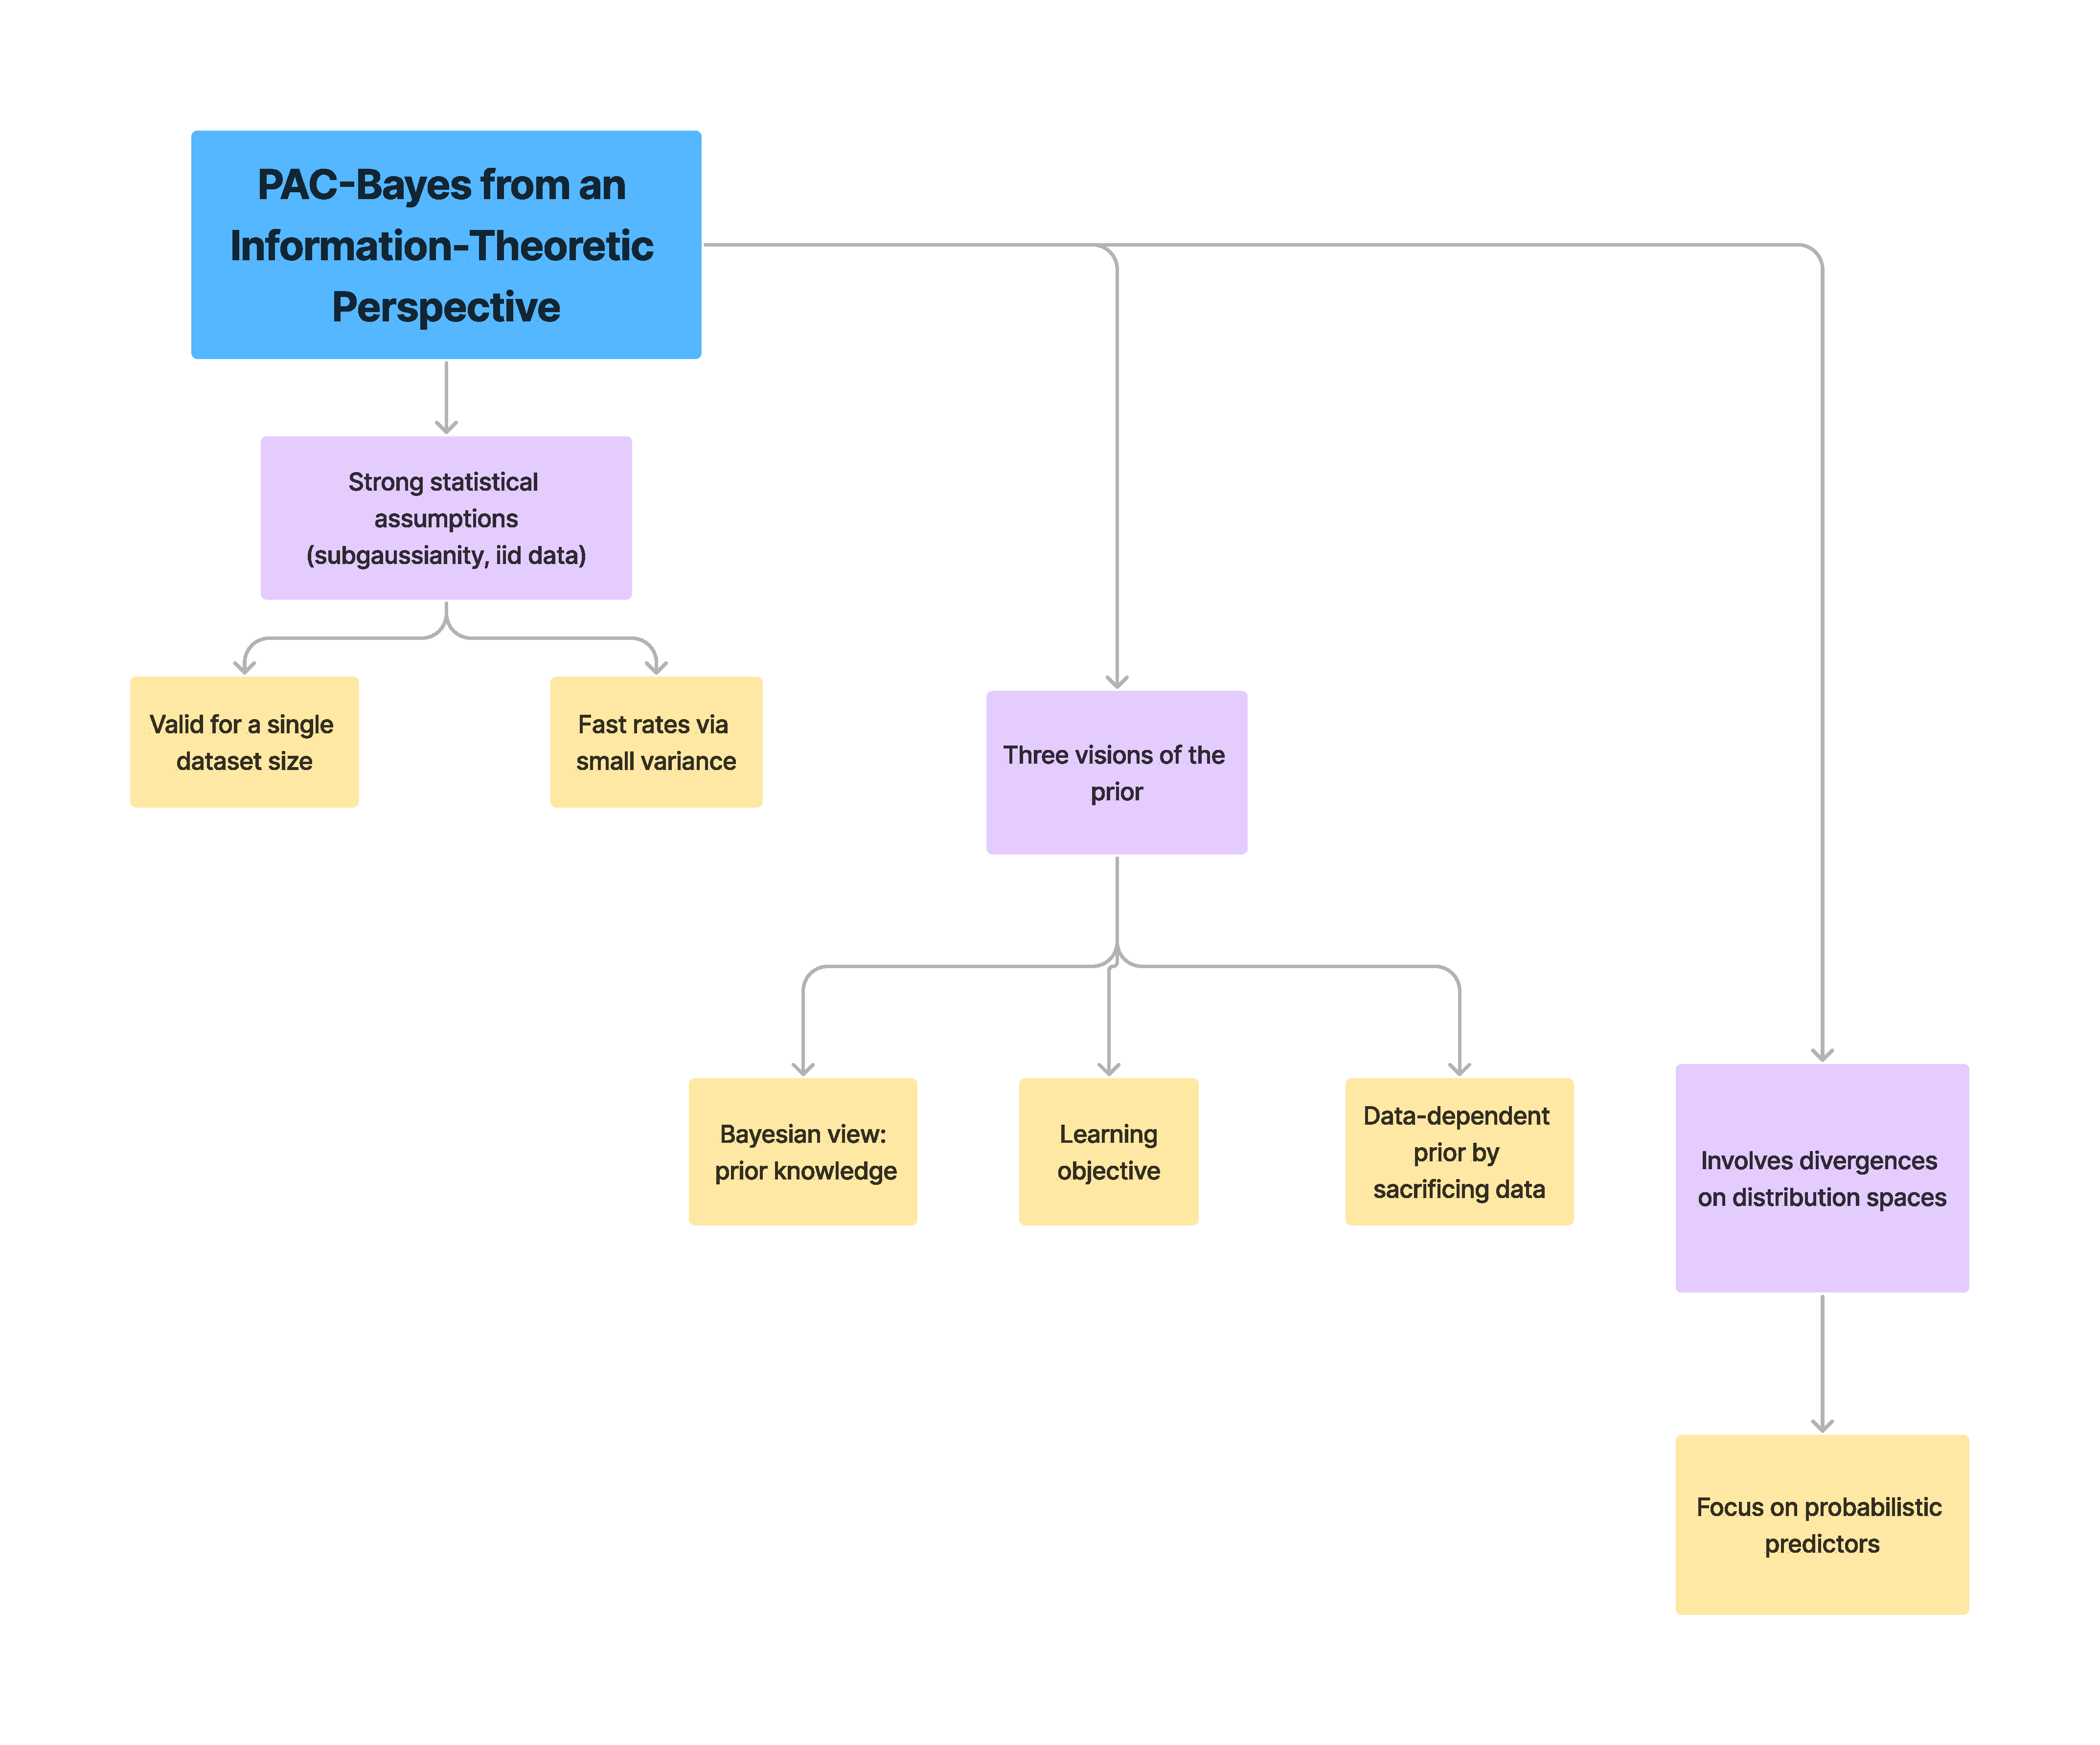
\includegraphics[scale=0.14]{recap-info.pdf}
    \end{figure}
  \end{xframe}

\begin{xframe}{A gap between Information Theory and practical Optimisation}
    \begin{block}{An elementary example}
        Training a deep neural net via SGD on a certain $\Sm$.
    \end{block}
\vspace{0.5cm}
{\bf To perform this optimisation}
    \begin{itemize}
        \item No statistical assumption is needed
        \item Random initialisation (no prior knowledge)
        \item Use of deterministic predictors (elements of $\Hcal$ not $\Mcal(\Hcal)$)
    \end{itemize}
    \vspace{0.5cm}
    \uncover<2->{\red{\bf \Large None of these fits the basic information-theoretic PAC-Bayes approach !}}\\
    \vspace{0.5cm}
    \uncover<3->{\orange{\bf \Large Can we think PAC-Bayes learning from an optimisation perspective? }}
\end{xframe}

\begin{xframe}{Towards an optimisation perspective}
    \vspace{1cm}
    \begin{itemize}
        \item \textbf{Existing attempts:} mix up PAC-Bayes with geometric properties of optimisation procedures (SGD, Langevin dynamics,...)  \citep{london2017pac,dziugaite2018entropy,neu2021info,clerico2022generalisation,haghifam2023limit,zhou2023toward} $\rightarrow$ new convergence properties, minimax rates.
        \item \green{\bf Contribution of this thesis:} propose general principles to derive novel bounds fitted with current practice in optimisation.
    \end{itemize}
    \vspace{0.5cm}


    \uncover<2->{{\blue{\Large To broadly sum up:}}\\\vspace{0.5cm}{\bf \Large Optimisation-driven PAC-Bayes aims to develop theory from practical constraints, Information theoretic PAC-Bayes tends to the opposite.}}

\end{xframe}

  \begin{xframe}{Contribution: PAC-Bayes with an Optimisation Perspective }
    \begin{figure}
        \centering
        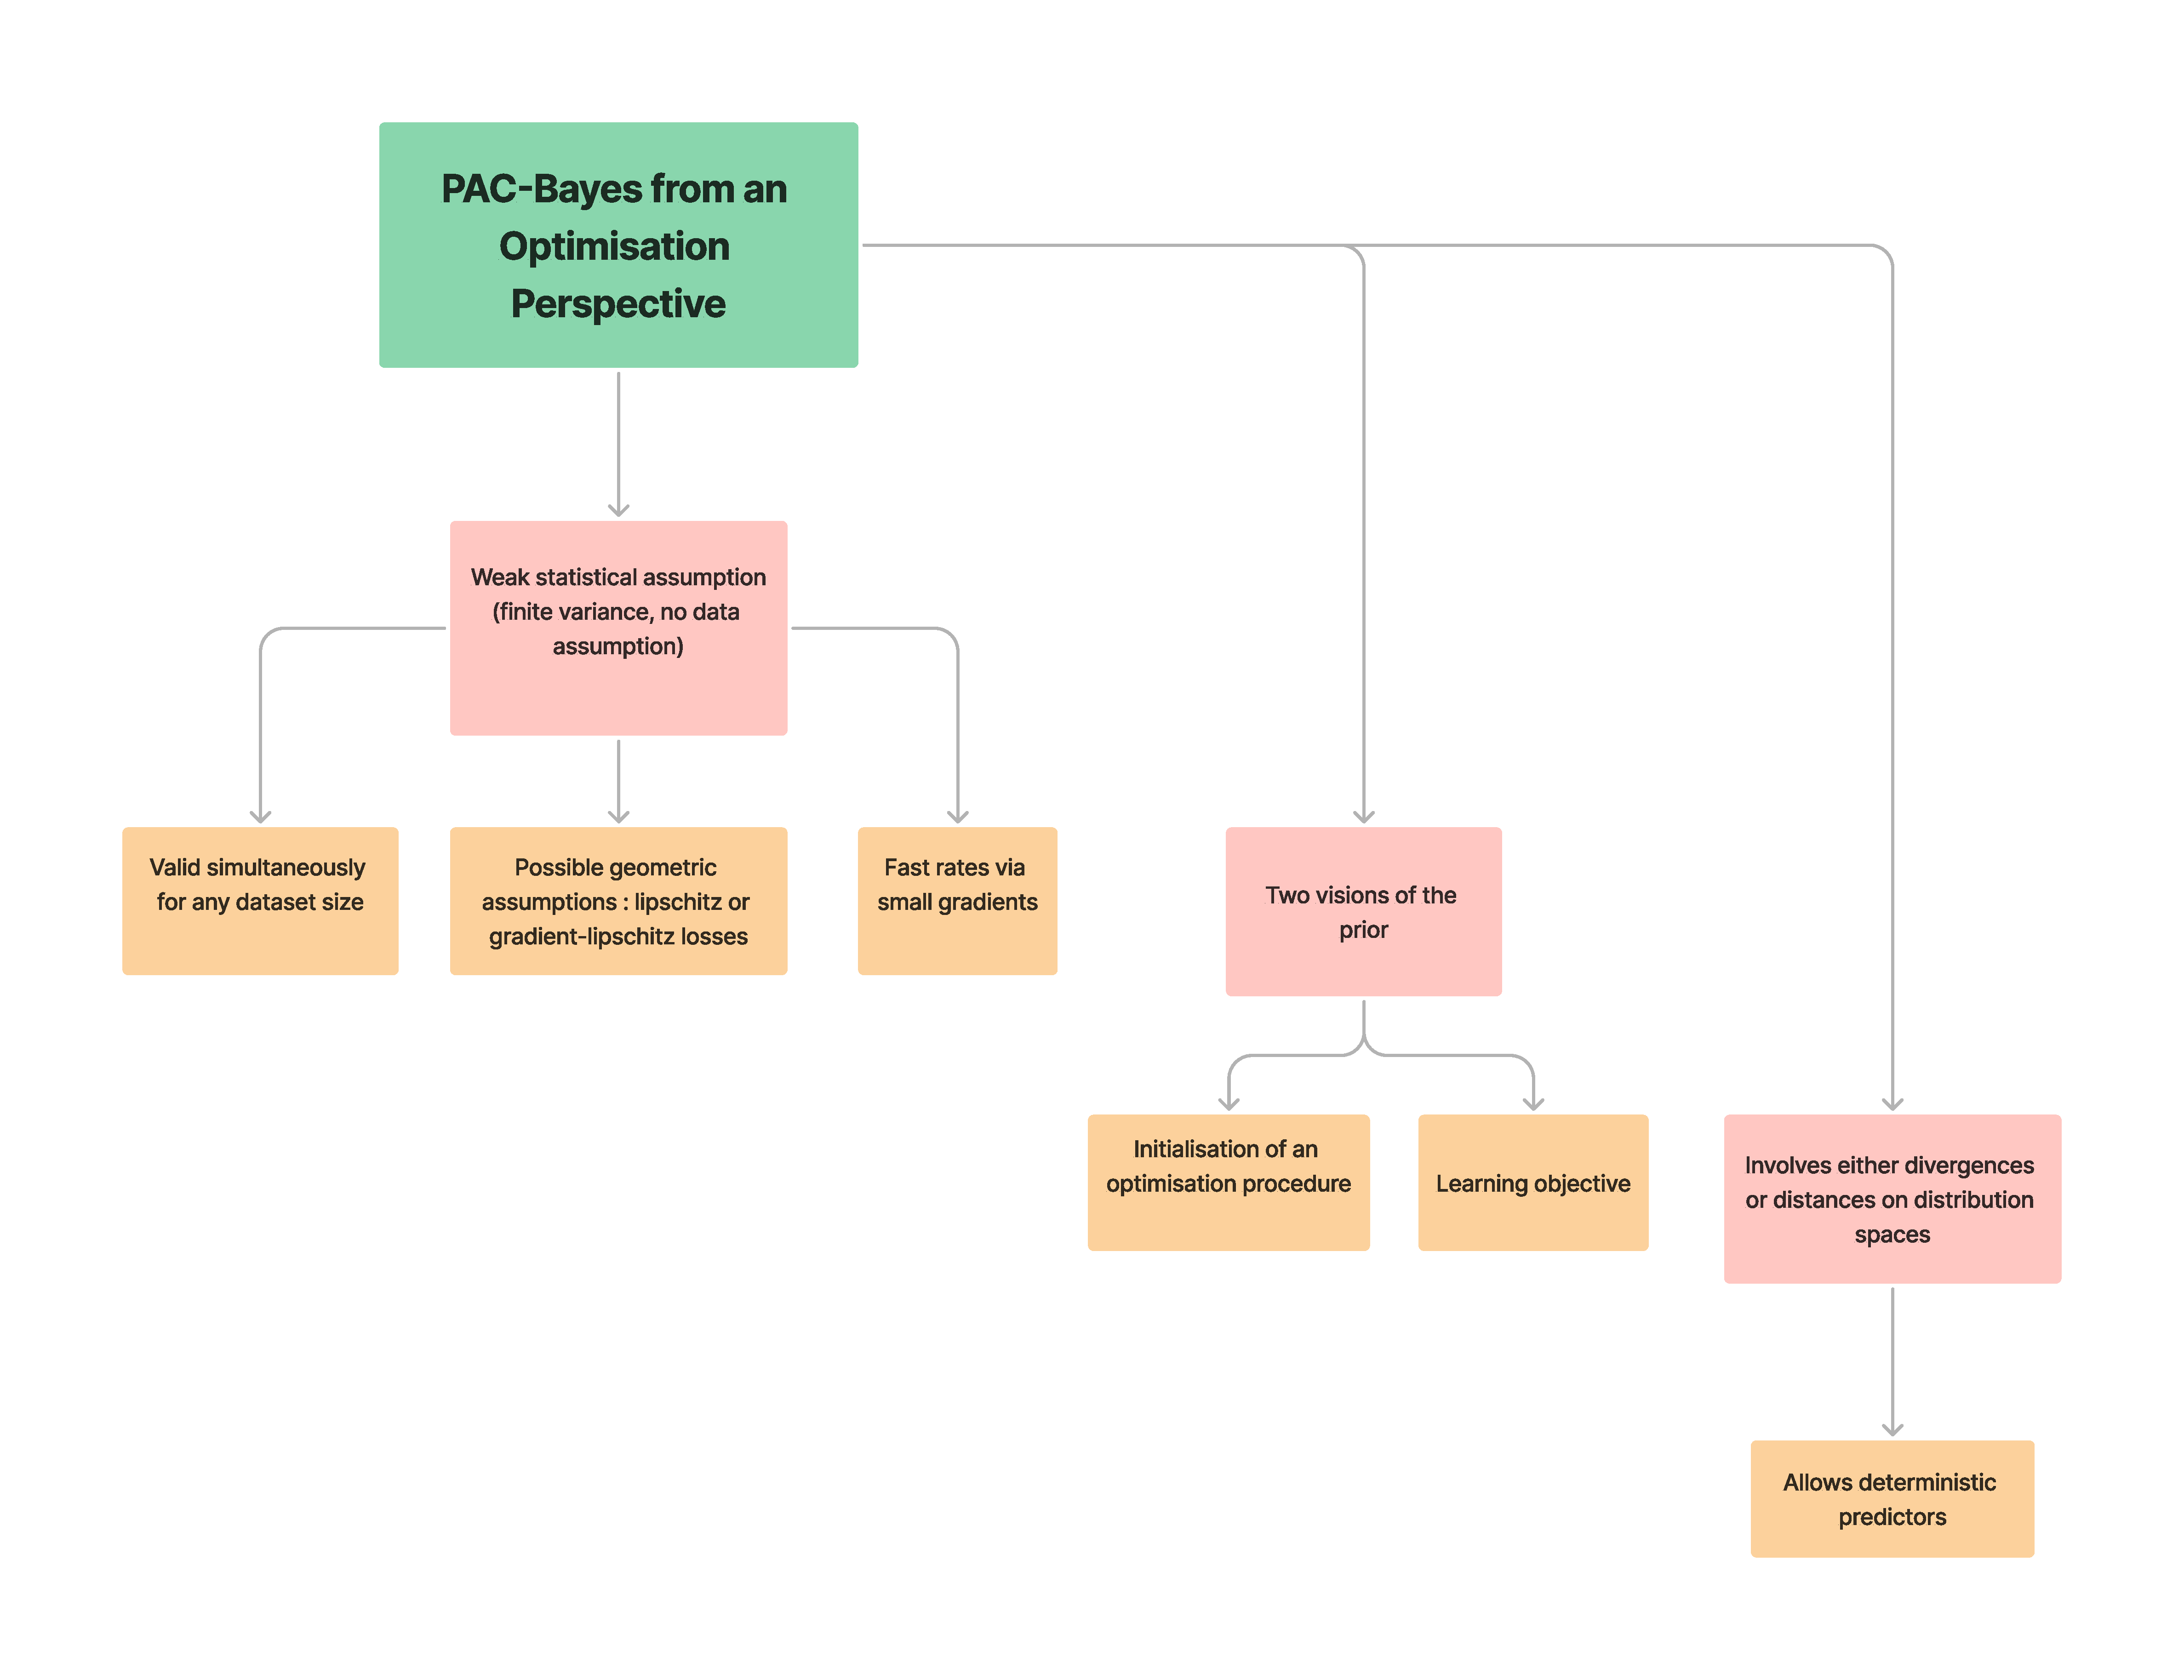
\includegraphics[scale=0.14]{recap-optim.pdf}
    \end{figure}
  \end{xframe}


\section{PAC-Bayes with Weak Statistical Assumptions}

\begin{xframe}{PAC-Bayes with Weak Statistical Assumptions}
  \begin{figure}
      \centering
      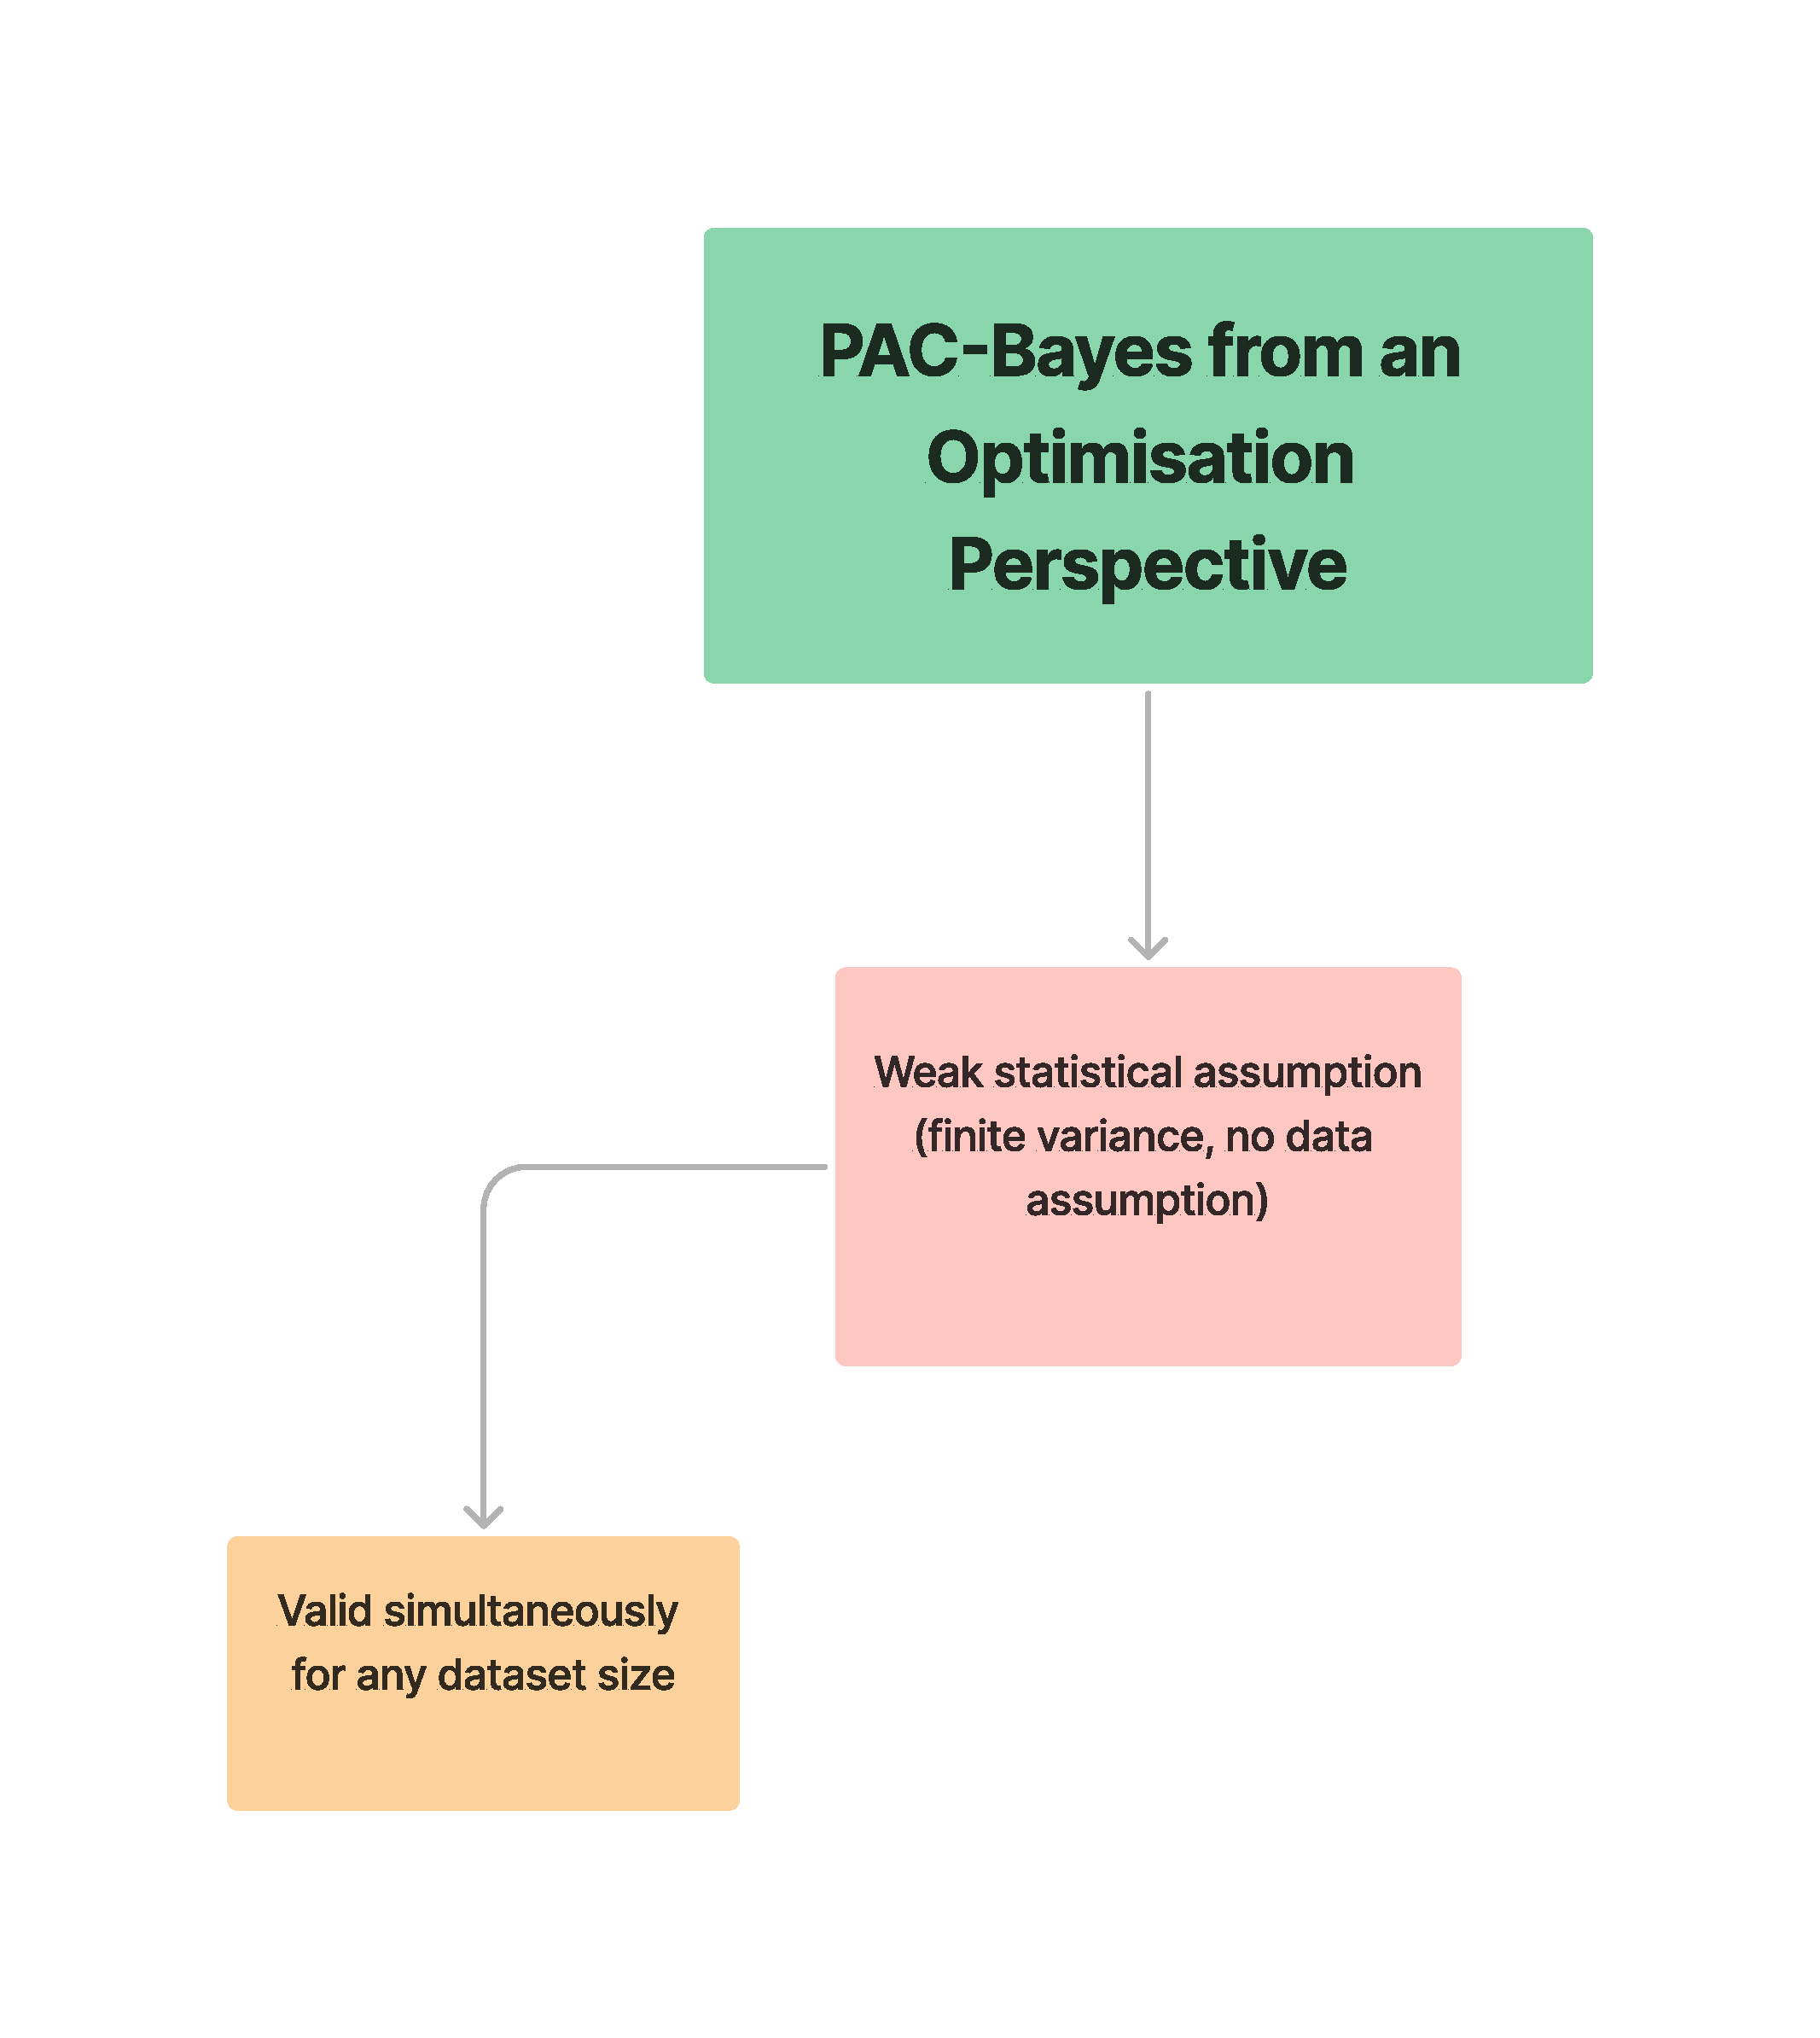
\includegraphics[scale=0.14]{diagram-chap-2.pdf}
  \end{figure}
\end{xframe}

\begin{xframe}{Weakening the subgaussian assumption}
    \vspace{0.5cm}
    \begin{itemize}
        \item Classical PAC-Bayes bounds assume \iid $\Sm$ and the loss either bounded, subgaussian or subexponential (few exceptions \eg: \citealp{audibert2011robust,seldin2012pac,alquier2018simpler} among others)
        \item In particular: \citet{kuzborskij2019efron} considered only finite variance assumption for independent $\Sm$.
    \end{itemize}
    \vspace{0.5cm}
    \green{\bf \Large Contribution: New PAC-Bayes bounds for any dataset $\S$ and finite variance assumption} 
    
\end{xframe}

\begin{xframe}{A PAC-Bayesian bound for unbounded martingales}
    
    \begin{blueblock}{\bf Theorem}
        For any data-free prior $\P\in \mathcal{M}(\mathcal{H})$, any $\lambda>0$, any collection of martingales $(M_m(h))_{m\geq 1}$ indexed by $h\in\mathcal{H}$, the following holds with probability $1-\delta$ over the sample $\S=(\z_i)_{i\in\mathbb{N}}$, for all $m\in\mathbb{N}/\{0\}$, $\Q\in\mathcal{M}(\mathcal{H})$:
\[|M_m(\Q)| \leq   \frac{\operatorname{KL}(\Q,\P) +\log(2/\delta)}{\lambda } + \frac{\lambda}{2}\left([M]_m(\Q) + \langle M\rangle_m(\Q) \right).  \]
    \end{blueblock}
\vspace{0.5cm}

\uncover<2->{\green{Novelty: no assumption on the $(M_m)_{m\geq 1}$ except the finiteness of $([M_m],\langle M\rangle_m)_{m\geq 1}$  and holds uniformly on all $m\geq 1$ }\\
\vspace{0.5cm} 
Toolbox: Ville's inequality and supermartingales}
\end{xframe}

\begin{xframe}{Instantiation}
    \vspace{0.5cm}
    A crucial particular case: batch learning with \iid $\S$\\
    \vspace{0.3cm}
    \begin{blueblock}{\bf Corollary}
        For any data-free prior $P\in \mathcal{M}(\mathcal{H})$, any $\lambda>0$ and $\ell\geq 0$, the following holds with probability $1-\delta$ over the sample $\S=(\z_i)_{i\in\mathbb{N}}$, for all $m\in\mathbb{N}/\{0\}$, $Q\in\mathcal{M}(\mathcal{H})$
\begin{multline*}\mathbb{E}_{h\sim \Q} [\Risk(h)] \leq   \mathbb{E}_{h\sim \Q} \left[\Riskhat_{\Sm}(h) + \frac{\lambda}{2m}\sum_{i=1}^m \ell(h,z_i)^2\right] \\
  + \frac{\operatorname{KL}(\Q,\P) +\log(2/\delta)}{\lambda m} + \frac{\lambda}{2}\mathbb{E}_{h\sim \Q} [\mathrm{Quad}(h)],
\end{multline*}
where $Quad(h)= \mathbb{E}_{\z\sim\D}[\ell(h,z)^2]$.
    \end{blueblock}
\end{xframe}

\begin{xframe}{Take-home message}
    \vspace{1cm}
    A first step towards the optimisation perspective of PAC-Bayes by weakening statistical assumptions. \\
    
    \vspace{1cm}However, we're still close from information theory: 
    \begin{enumerate}
        \item $\P$ does not fit the optimisation view of the prior  
        \item KL term remains close from information theory.
    \end{enumerate}
    \vspace{1cm}
    {\orange{\bf \Large How do we deal with those inquiries?}}
    \vspace{0.5cm}
\end{xframe}


\section{Mitigating Initialisation Impact by Real-Time Control: Online PAC- Bayes Learning}

\begin{xframe}{Mitigating Initialisation Impact: Online PAC- Bayes Learning}
    \begin{figure}
        \centering
        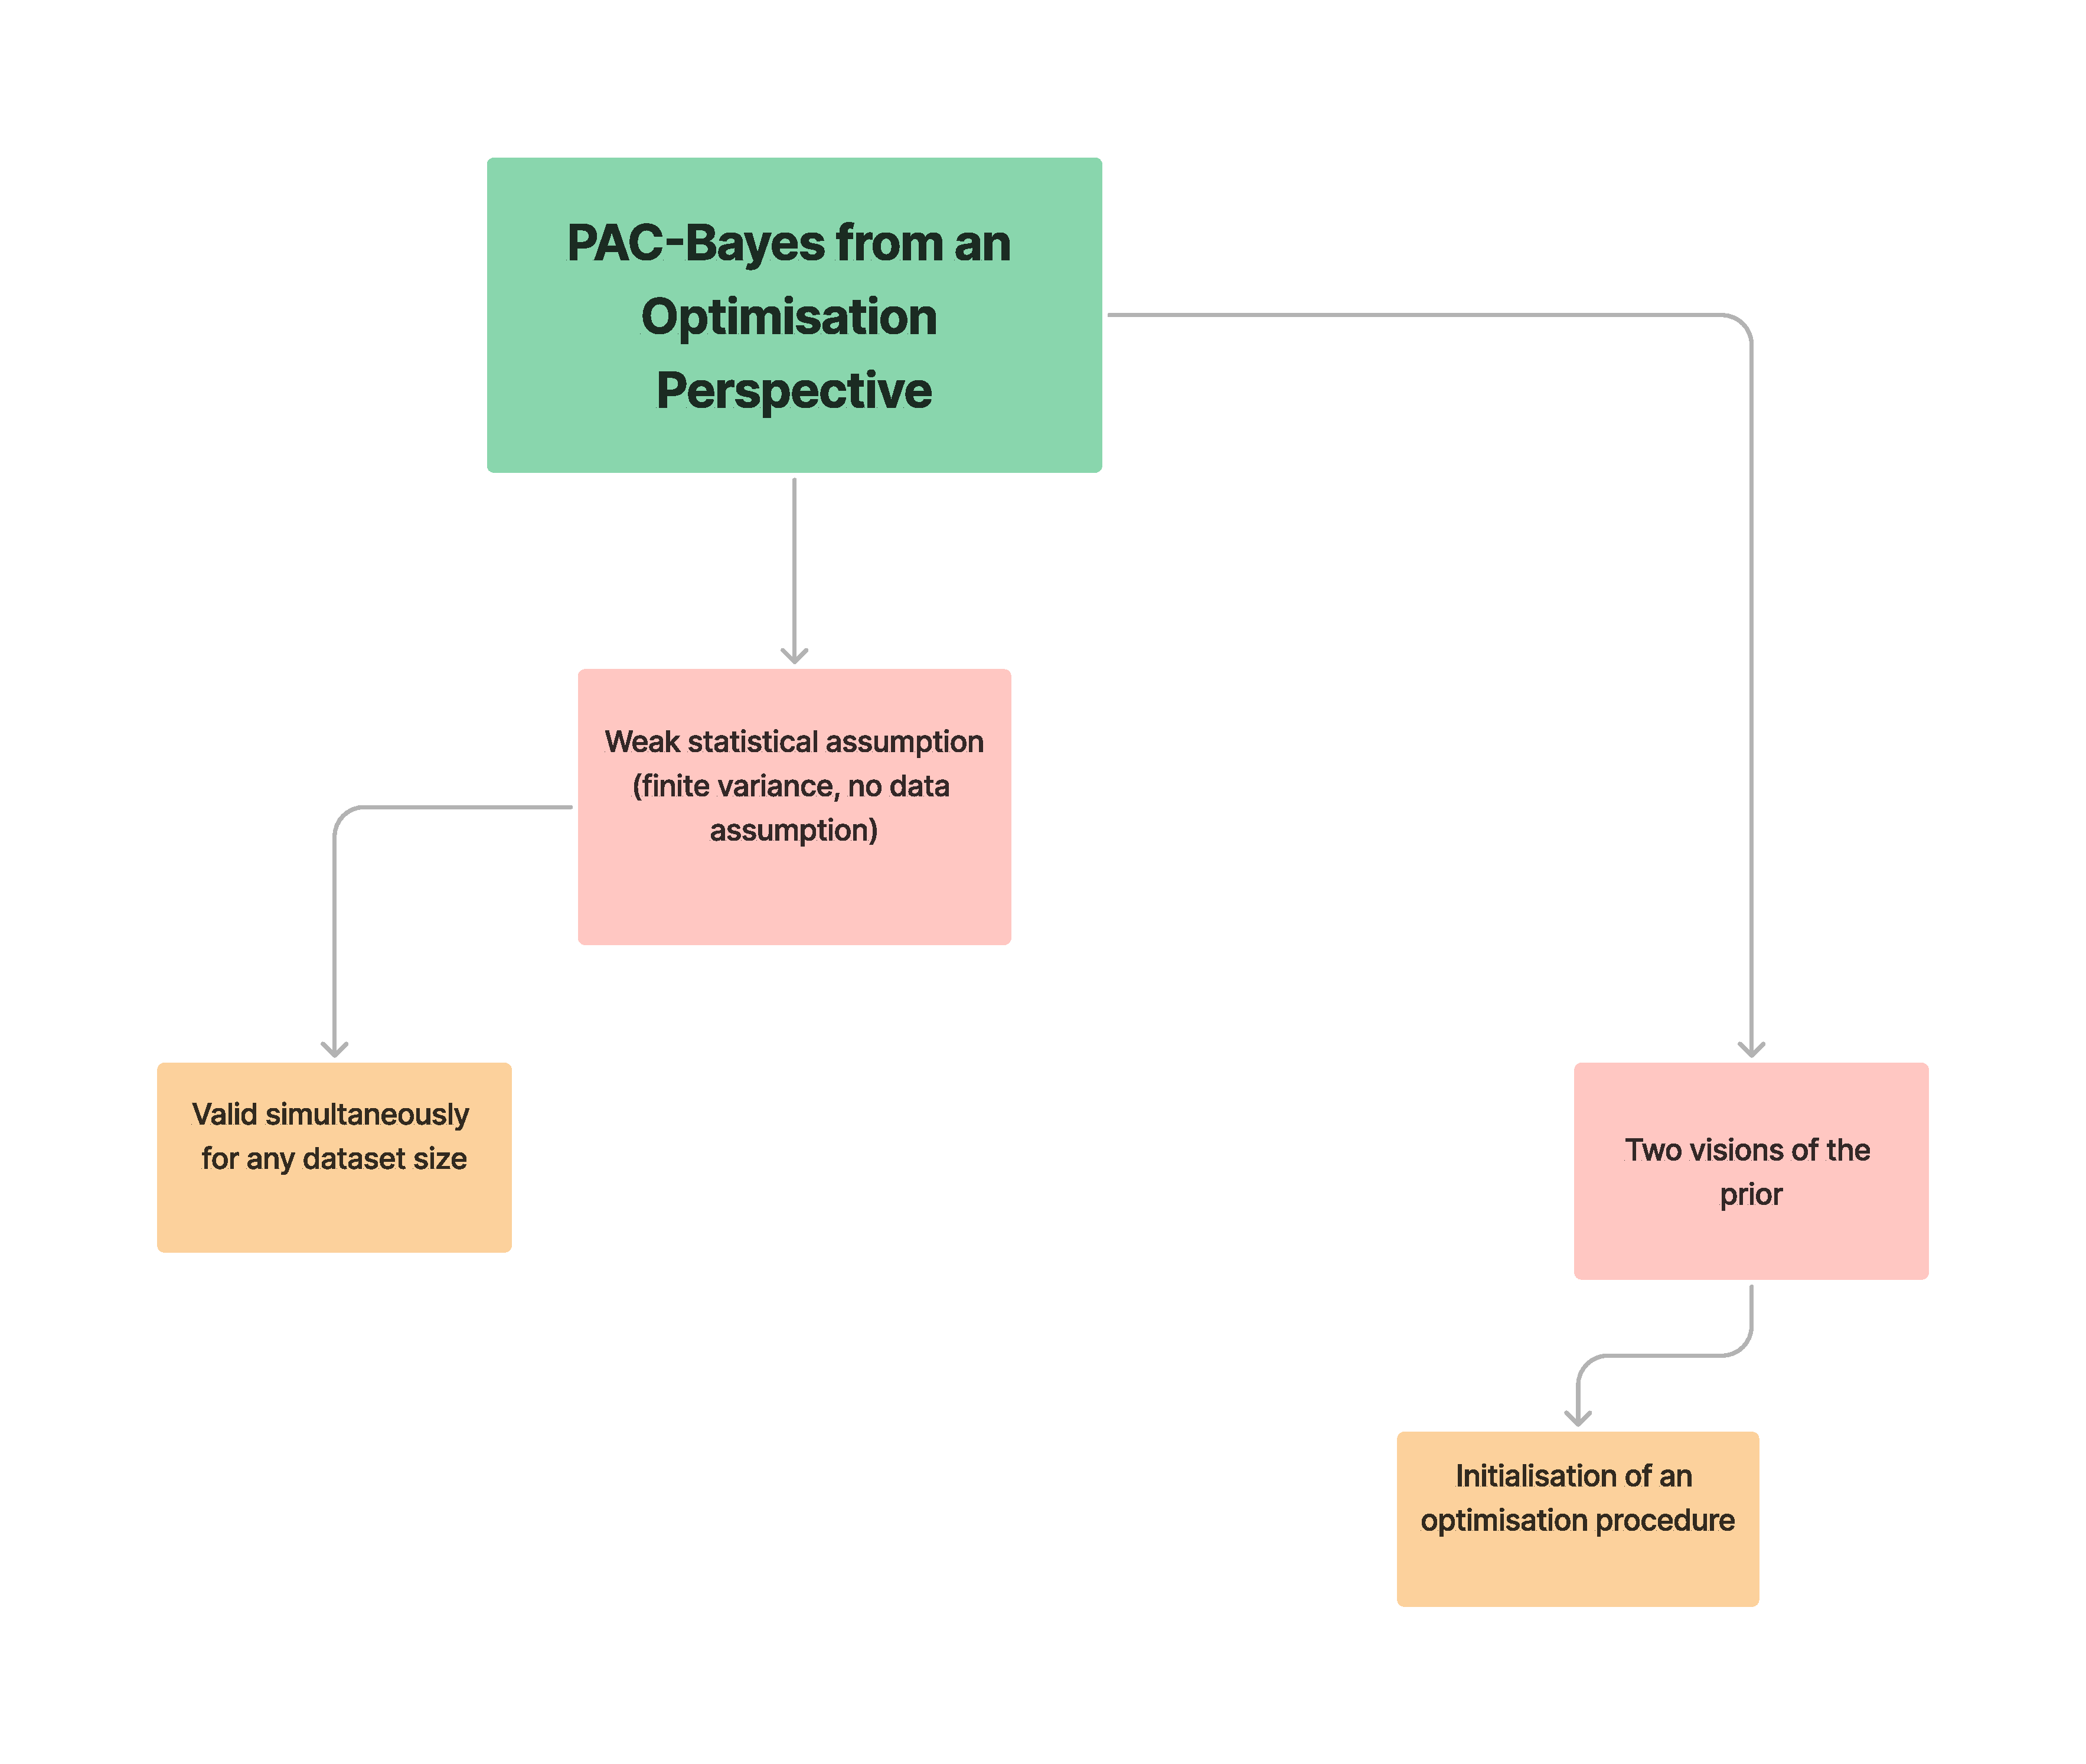
\includegraphics[scale=0.14]{diagram-chap-3.pdf}
    \end{figure}
  \end{xframe}

  \begin{xframe}{Prior as initialisation point}
    \vspace{0.5cm}
    {\blue{\bf \Large Usually, $\P$ is a regulariser containing prior information}}
    \vspace{0.5cm}
    {\red{\bf \Large Practical issue: no clue in choice of $\P$ (used as initialisation),$\rightarrow$ regularisation may harm learning}}
    \vspace{0.5cm}
    {\orange{\bf \Large In this case, can we reduce the impact of $\P$ in PAC-Bayes training?}}
    \vspace{0.5cm}

    {\green{\bf \Large Yes, thanks to Online Learning, which allows to consider an evolving sequence of priors $(\P_i)_{i\geq 1}$ ! }\\
    
    \begin{block}{\bf Additional Setting}
        $(\mathcal{F}_i)_{i\geq 1}$ is a filtration adapted to $\S$ and $\P_i$ is said to be an \emph{online predictive sequence} if for all $i$, $\P_i$ is a stochastic kernel $\mathcal{F}_{i-1}$ measurable and for all $i$, $\P_i \ll \P_1$.
    \end{block}}

  \end{xframe}

  \begin{xframe}{An online PAC-Bayesian bound for heavy-tailed losses}

    \begin{blueblock}{\bf Theorem}
        For any distribution $\D_\S$, any $\lambda>0$ and any online predictive sequence $(\P_{i})_{i\geq 1}$, with probability at least $1-\delta$ over $\S$ the following, holding for the sequence $\P_{i,\S}:= \P_{i}(\S,.)$, any posterior sequence $(\Q_{i})_{i\geq 1}$ and any $m\geq 1$:

  \begin{multline*}
     \sum_{i=1}^m \mathbb{E}_{h_i\sim \Q_{i}}\left[ \mathbb{E}[\ell(h_i,\z_i) \mid \mathcal{F}_{i-1}]    \right]  \leq \sum_{i=1}^m \mathbb{E}_{h_i\sim \Q_{i}}\left[ \ell(h_i,\z_i) \right] \\+\frac{\lambda}{2}\sum_{i=1}^m \mathbb{E}_{h_i\sim \Q_{i}}\left[ \hat{V}_i(h_i,\z_i) + V_i(h_i) \right]
     + \sum_{i=1}^m\frac{\operatorname{KL}(\Q_{i}, \P_{i,\S})}{\lambda}  + \frac{\log(1/\delta)}{\lambda}.
  \end{multline*}
  With for all $i$, $\hat{V}_i(h_i,\z_i)= (\ell(h_i,\z_i)-\mathbb{E}_{i-1}[\ell(h_i,\z_i)])^2$ is the empirical variance at time $i$ and $V_i(h_i)= \mathbb{E}_{i-1}[\hat{V}(h_i,\z_i)]$ is the true conditional variance.
    \end{blueblock}
   
    
  \end{xframe}

  \begin{xframe}{A corollary for bounded variance}
    Assuming variance terms uniformly bounded by $K^2/2$ (strictly weaker than assuming bounded losses) gives :

    \begin{blueblock}{\bf Corollary}
        For any distribution $\D_\S$, any $\lambda>0$ and any online predictive sequence $(\P_{i})_{i\geq 1}$, with probability at least $1-\delta$ over $\S$ the following, holding for the sequence $\P_{i,\S}:= \P_{i}(\S,.)$, any posterior sequence $(\Q_{i})_{i\geq 1}$ and any $m\geq 1$:

  \begin{multline*}
     \sum_{i=1}^m \mathbb{E}_{h_i\sim \Q_{i}}\left[ \mathbb{E}[\ell(h_i,\z_i) \mid \mathcal{F}_{i-1}]    \right]  \leq \sum_{i=1}^m \mathbb{E}_{h_i\sim \Q_{i}}\left[ \ell(h_i,\z_i) \right] \\
     + \sum_{i=1}^m\frac{\operatorname{KL}(\Q_{i}, \P_{i,\S})}{\lambda}  +\frac{\lambda mK^2}{2} + \frac{\log(1/\delta)}{\lambda}.
  \end{multline*}
    \end{blueblock}
  \end{xframe}

  \begin{xframe}{An Online PAC-Bayesian procedure}
    \vspace{0.5cm}
    \begin{align*}
        \hat{\Q}_1= \P_1, \quad \forall i\geq1\; \hat{\Q}_{i+1}&= \underset{Q\in\mathcal{M}(\mathcal{H})}{\mathrm{argmin}} \mathbb{E}_{h_i\sim \Q} \; [\ell(h_i,\z_i)] + \frac{\operatorname{KL}(\Q, \P_{i})}{\lambda} \\
        \intertext{which leads to the explicit formulation}
        \frac{d\hat{\Q}_{i+1}}{d\P_{i}}(h)& = \frac{\exp\left(-\lambda  \ell(h,\z_i)\right)}{\mathbb{E}_{h\sim \P_{i}}\left[\exp\left(-\lambda  \ell(h,\z_i)\right)\right]}.
      \end{align*}

      \uncover<2->{\vspace{0.5cm}
      {\red{\bf \Large Drawback: Gibbs posteriors are costful to implement}}\\
      \vspace{0.5cm}
      {\green{\bf \Large Solution: Disintegrated Online PAC-Bayes Algorithm}}}


  \end{xframe}

  \begin{xframe}{Practice}
    Disintegrated algorithm in a nutshell : $\hat{\Q}_i= \mathcal{N}(\hat{w}_i,\sigma^2 \mathrm{Id})$ and:
    \[ \hat{w}_{i+1}:= \operatorname{argmin}_{w\in\mathbb{R}^d} \ell(w + \varepsilon_i,z_i) + \Psi(w+ \varepsilon_i,w, w_i^0)   \]

    \begin{figure}
        \centering
        \includegraphics[scale=0.4]{online-pb.png}
    \end{figure}
    
  \end{xframe}

  \begin{xframe}{Take-home messages}
    \vspace{0.5cm}
    {\green{\Large\bf Success: Online PAC-Bayes mitigates the impact of the prior, seen as an initialisation point, yielding performances at least comparable to online gradient descent. }}\\
    \vspace{1cm}
    {\orange{\Large\bf However, two questions remain open: }}

    \begin{enumerate}
        \item Is it possible to propagate the view of prior as initialisation directly for batch algorithms?
        \item Is it possible to obtain PAC-Bayes learning algorithms directly for deterministic predictors instead of using disintegrated results in order to be consistent with practitioners, often avoiding stochastic predictors?
    \end{enumerate}
    
  \end{xframe}

%Detail Online PAC-Bayes bounds alongside algorithmic results

\section{Mitigating Initialisation Impact through Flat Minima: Fast Rates for Small Gradients}

\begin{xframe}{Mitigating Initialisation Impact: Fast Rates for Small Gradients}
    \begin{figure}
        \centering
        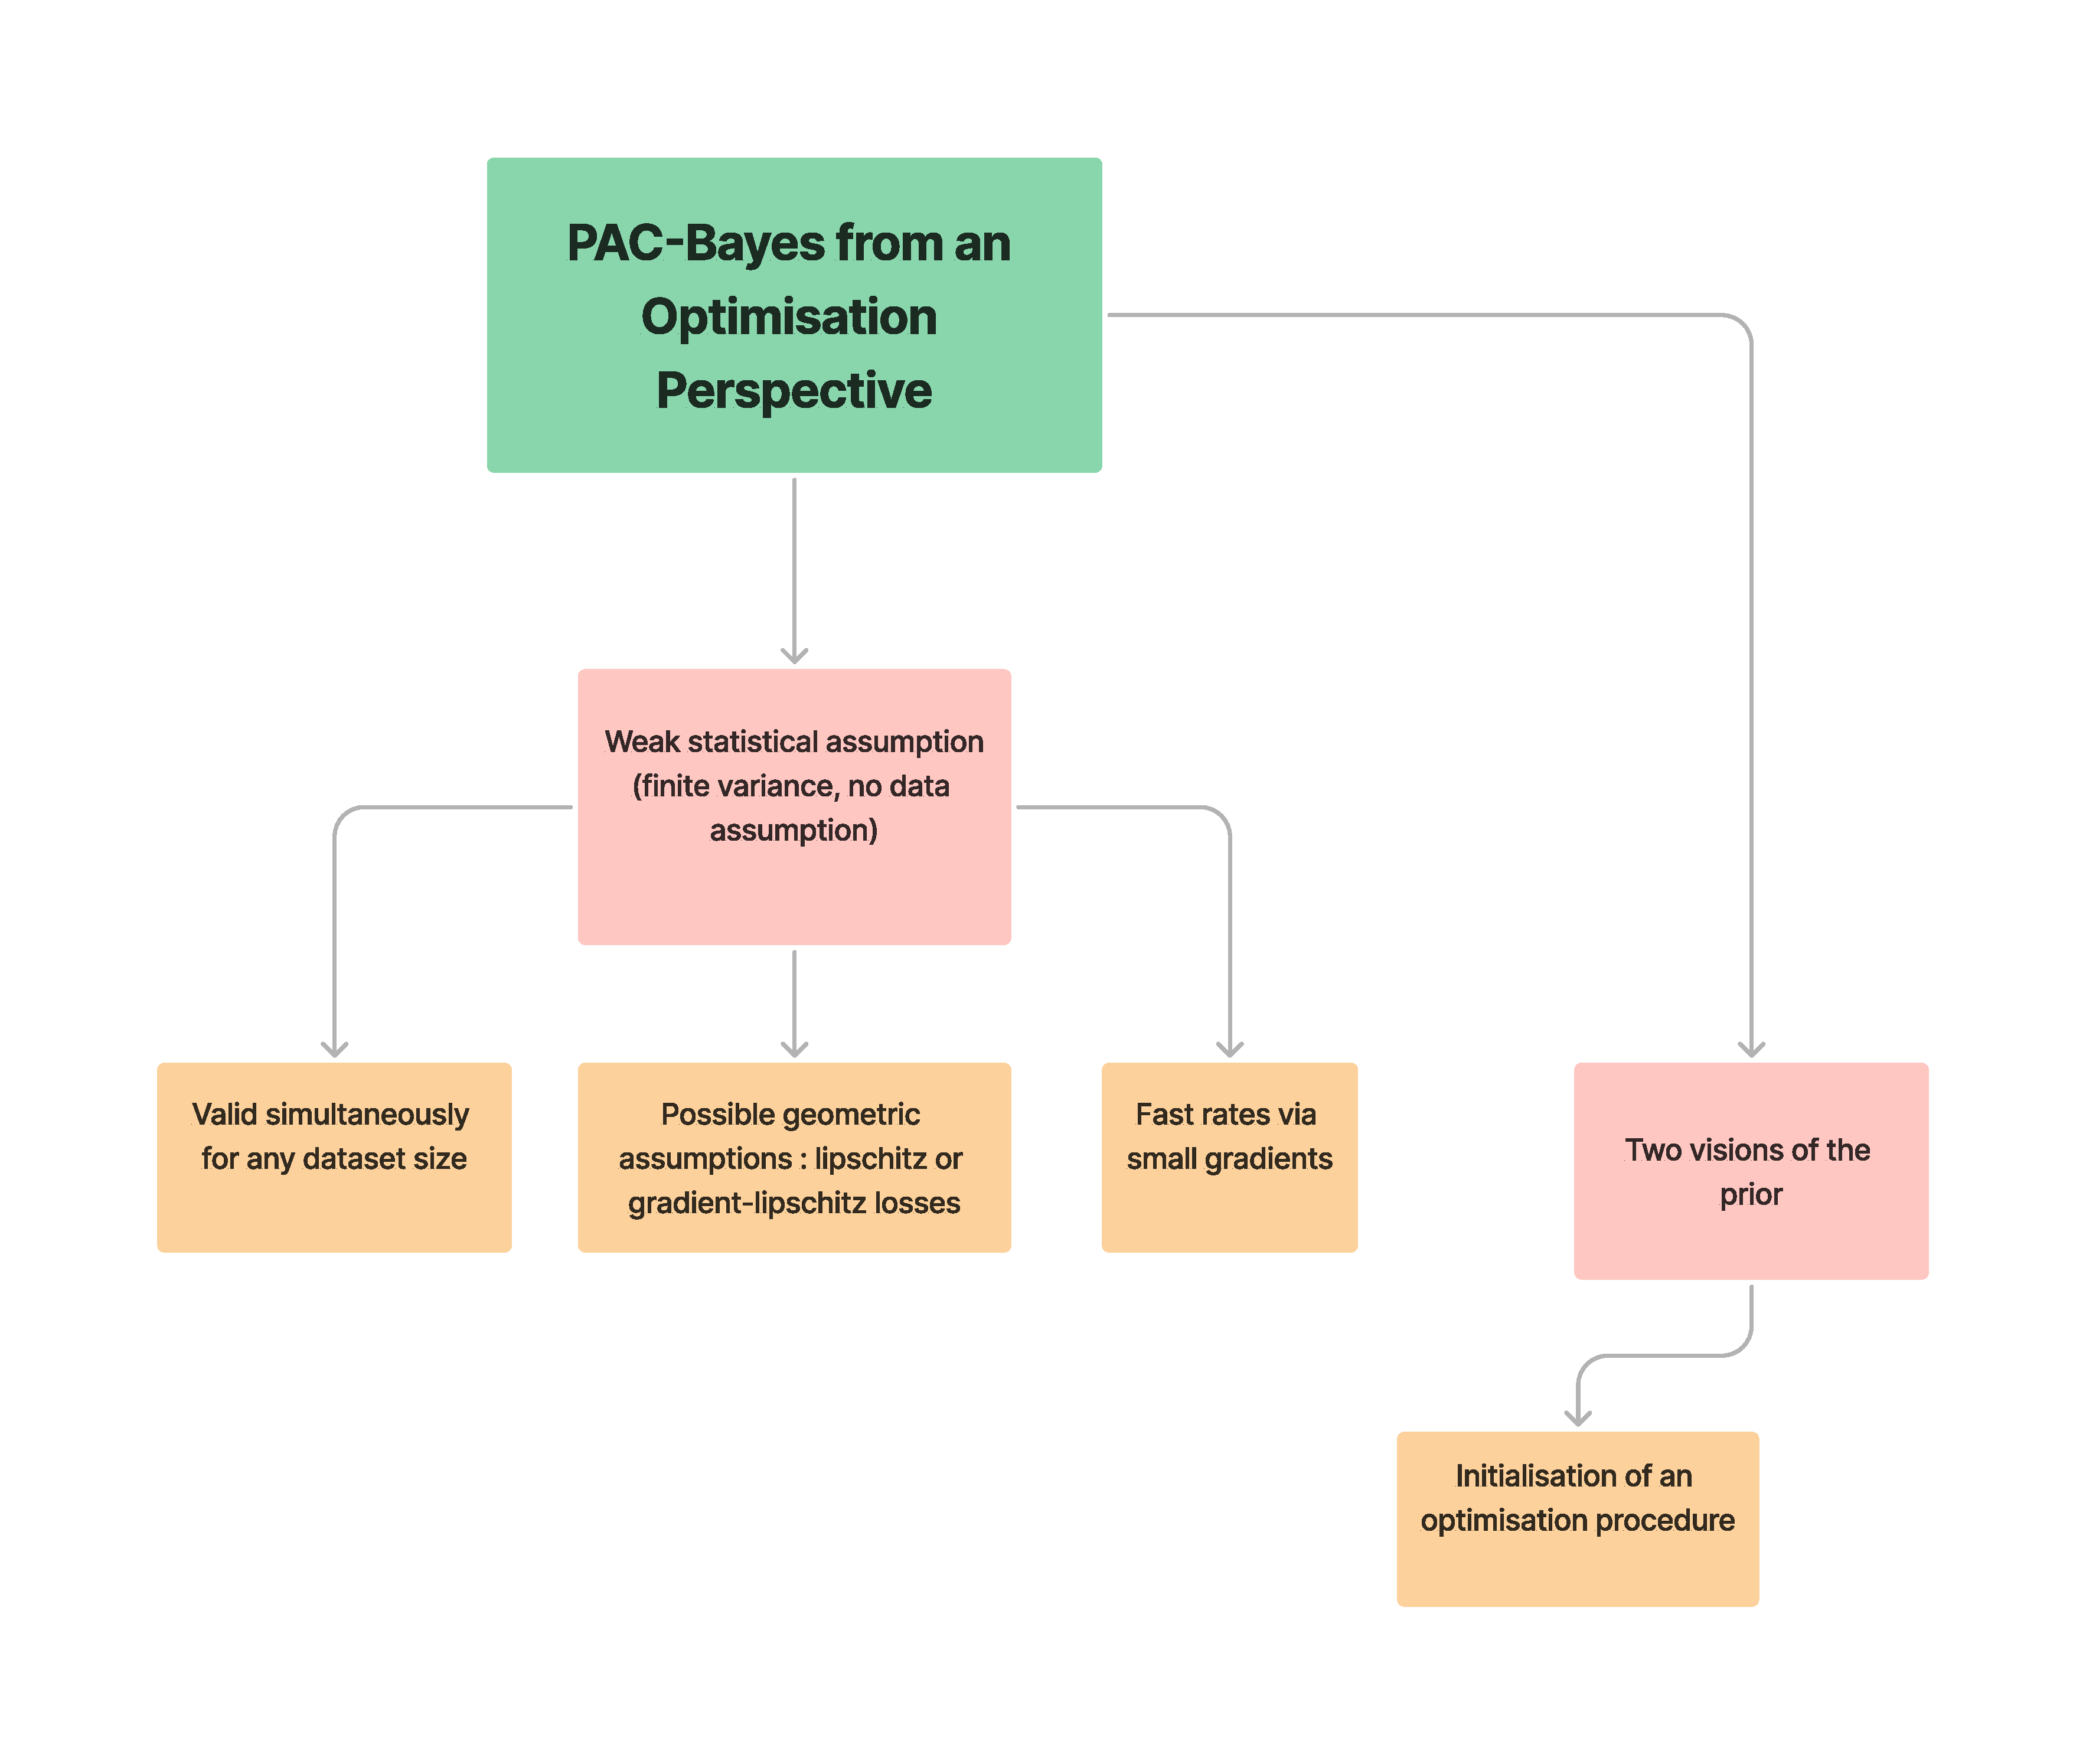
\includegraphics[scale=0.14]{diagram-chap-4.pdf}
    \end{figure}
  \end{xframe}

%Shrink this section
\begin{xframe}{Flat minimum}
    \textbf{What is a flat minimum?}
    \\
  \blue{A minimum such that its neighbourhood nearly minimises the loss.}
    \vspace{1cm}
    \begin{figure}
        \includegraphics[scale= 0.5]{figures/flat-minima.png} 
    \end{figure}
{\tiny Image from \citet{liebenwein2021sparse}. }
\end{xframe}




\begin{xframe}{Fast-rate generalisation bounds for flat minima (1)}
  \small{\green{Notation:} $\Err(\ell,\Q,\z):= \EE_{h\sim\Q}[\ell(h,\z)]$}
    \vspace{1cm}
    \begin{block}{\textbf{Assumption}}
    $\Q\in\Mcal(\Hcal)$ is \emph{quadratically self-bounded} \wrt $\ell$ and  $C>0$ (namely $\texttt{QSB}(\ell,C)$) if
    \[ \mathbb{E}_{\z\sim \D}\LB \Err(\ell,\Q,\z)^2 \RB \leq C \Risk_\D(\Q) \LP = C\mathbb{E}_{\z\sim \D}\LB \Err(\ell,\Q,\z) \RB \RP   \]
    \end{block}
    \vspace{0.7cm}
    \begin{xitemize}
        \item QSB intricates $\D\in\Mcal(\Zcal)$ with $\Q \in \Mcal(\H)$
        \vspace{0.2cm}
        \item Satisfied if $\ell\in [0,K]$ with $C=K$.
        \vspace{0.2cm}
        \item \texttt{QSB} quantifies the 'flatness' of the post-training minima reached by $\Q$.
    \end{xitemize}
    
    
\end{xframe}

\begin{xframe}{Is the QSB assumption verified in practice?}
    \red{\textbf{QSB holds for 3-layer neural nets trained on MNIST (black curve)!}}
  \begin{figure}
      \centering
      \includegraphics[scale=0.4]{result-flat-minima.pdf}
  \end{figure}
\end{xframe}

\begin{xframe}{Fast-rate generalisation bounds via flat minima (2)}
    \vspace{1cm}
  \begin{blueblock}{\bf Theorem}
      For any $C>0$, data-free prior $\P$, with probability at least $1-\delta$ for any $m>0$, and $\Q$ being $\Poinc(c_P)$, $\texttt{QSB}(\ell,C)$,
      \begin{align*}
      \Risk_{\D}(\Q) \leq  2\hat{\Risk}_{\S}(\Q) + 2C\frac{KL(\Q,\P) +\log(1/\delta)}{ m}  
       + \frac{1}{C} c_{P}(\Q)\EE_{\z\sim\D} \LB \EE_{h\sim \Q}\LP \|\nabla_h \ell(h,\z)\|^2 \RP \RB .
    \end{align*}
  \end{blueblock}

  
\end{xframe}


\begin{xframe}{Fully empirical fast rate}
    \red{\textbf{Drawback: bound not empirical.}}
    \vspace{0.3cm}
    
    \green{\textbf{Solution: $\mathcal{C}^2$ gradient-lipschitz losses!}}
    
    \begin{blueblock}{\bf Theorem}
        For any $C_1,C_2,c>0$, with probability at least $1-\delta$, for any $m>0$, $\Q$ being $\Poinc(c_P)$ with constant $c$, $\texttt{QSB}(\ell,C_1)$, $\texttt{QSB}\LP\|\nabla_h \ell\|^2,C_2\RP$, 
  
    \begin{align*}
      \Risk_{\D}(\Q) \leq &\; 2 \hat{\Risk}_{\S}(\Q) + \mathcal{O}\left( \EE_{h\sim \Q}\LB \frac{1}{m}\sum_{i=1}^m \|\nabla_h\ell(h,\z_i)\|^2 \RB  + \frac{\KL(\Q,\P) +\log(1/\delta)}{m}\right).
    \end{align*}
    \end{blueblock}
    \vspace{0.5cm}
    \uncover<2->{\bf Those bounds: holds for Gaussian and Gibbs. Other results for Gibbs posteriors in the manuscript!}

\end{xframe}

\begin{xframe}{Result for deterministic predictors}
    \Large 
    \vspace{2.5cm}
    \red{\textbf{Drawback: results hold for probabilistic predictors}}
    
    \vspace{0.3cm}
    \uncover<2->{\green{\textbf{Solution: Exploit the 2-Wasserstein distance to obtain guarantees valid for deterministic predictors (Diracs) }}}

    
\end{xframe}

\begin{xframe}{Result}
\vspace{1cm}
\begin{blueblock}{\bf Theorem}
    Let $\delta\in(0,1)$ and $P\in\Mcal(\Hcal)$ a data-free prior.
Assume $\Hcal$ has a finite diameter $D>0$, $\ell\geq 0$ and that for any $m$, the generalisation gap $\Delta_{\S_m}$ is $G$ gradient-Lipschitz.
Assume that $\mathbb{E}_{h\sim\P}\Ebb_{\z\sim\D}[\ell(h,z)^2] \leq \sigma^2$, then the following holds with probability at least $1-\delta$, for any $m>0$ and any $\Q$:
\begin{align*}
    \Risk_D(\Q) \leq \hat{\Risk}_{\S_m}(\Q) + \frac{G}{2} W_2^2(\Q,\P) + \sqrt{\frac{2\sigma^2\log\LP \frac{1}{\delta} \RP}{m}} + D \mathbb{E}_{h\sim \Q}\LP \left\| \nabla_h \Risk_\D(h) - \nabla_h \hat{\Risk}_{\S_m}(h) \right\| \RP
\end{align*}
\end{blueblock}
 
\end{xframe}

\begin{xframe}{To sum up}
    \vspace{1cm}
    \Large
    \begin{xitemize}
        \item We mathematically quantify the impact of flat minima in generalisation: momentum in Catoni's bound!
        \item The \texttt{QSB} condition is verified on basic neural nets (classification) with constant $C$ sharper than 1! 
        \item Wasserstein distance allows to involve Dirac predictors
    \end{xitemize}
    \vspace{0.5cm}
    \orange{\bf\Large Can we draw deeper links between Wasserstein distances and PAC-Bayes? }
    
\end{xframe}

\section{Wasserstein PAC-Bayes: Exploiting Optimisation to Explain Generalisation}

\begin{xframe}{Wasserstein PAC-Bayes: From Optimisation to Generalisation}
    \begin{figure}
        \centering
        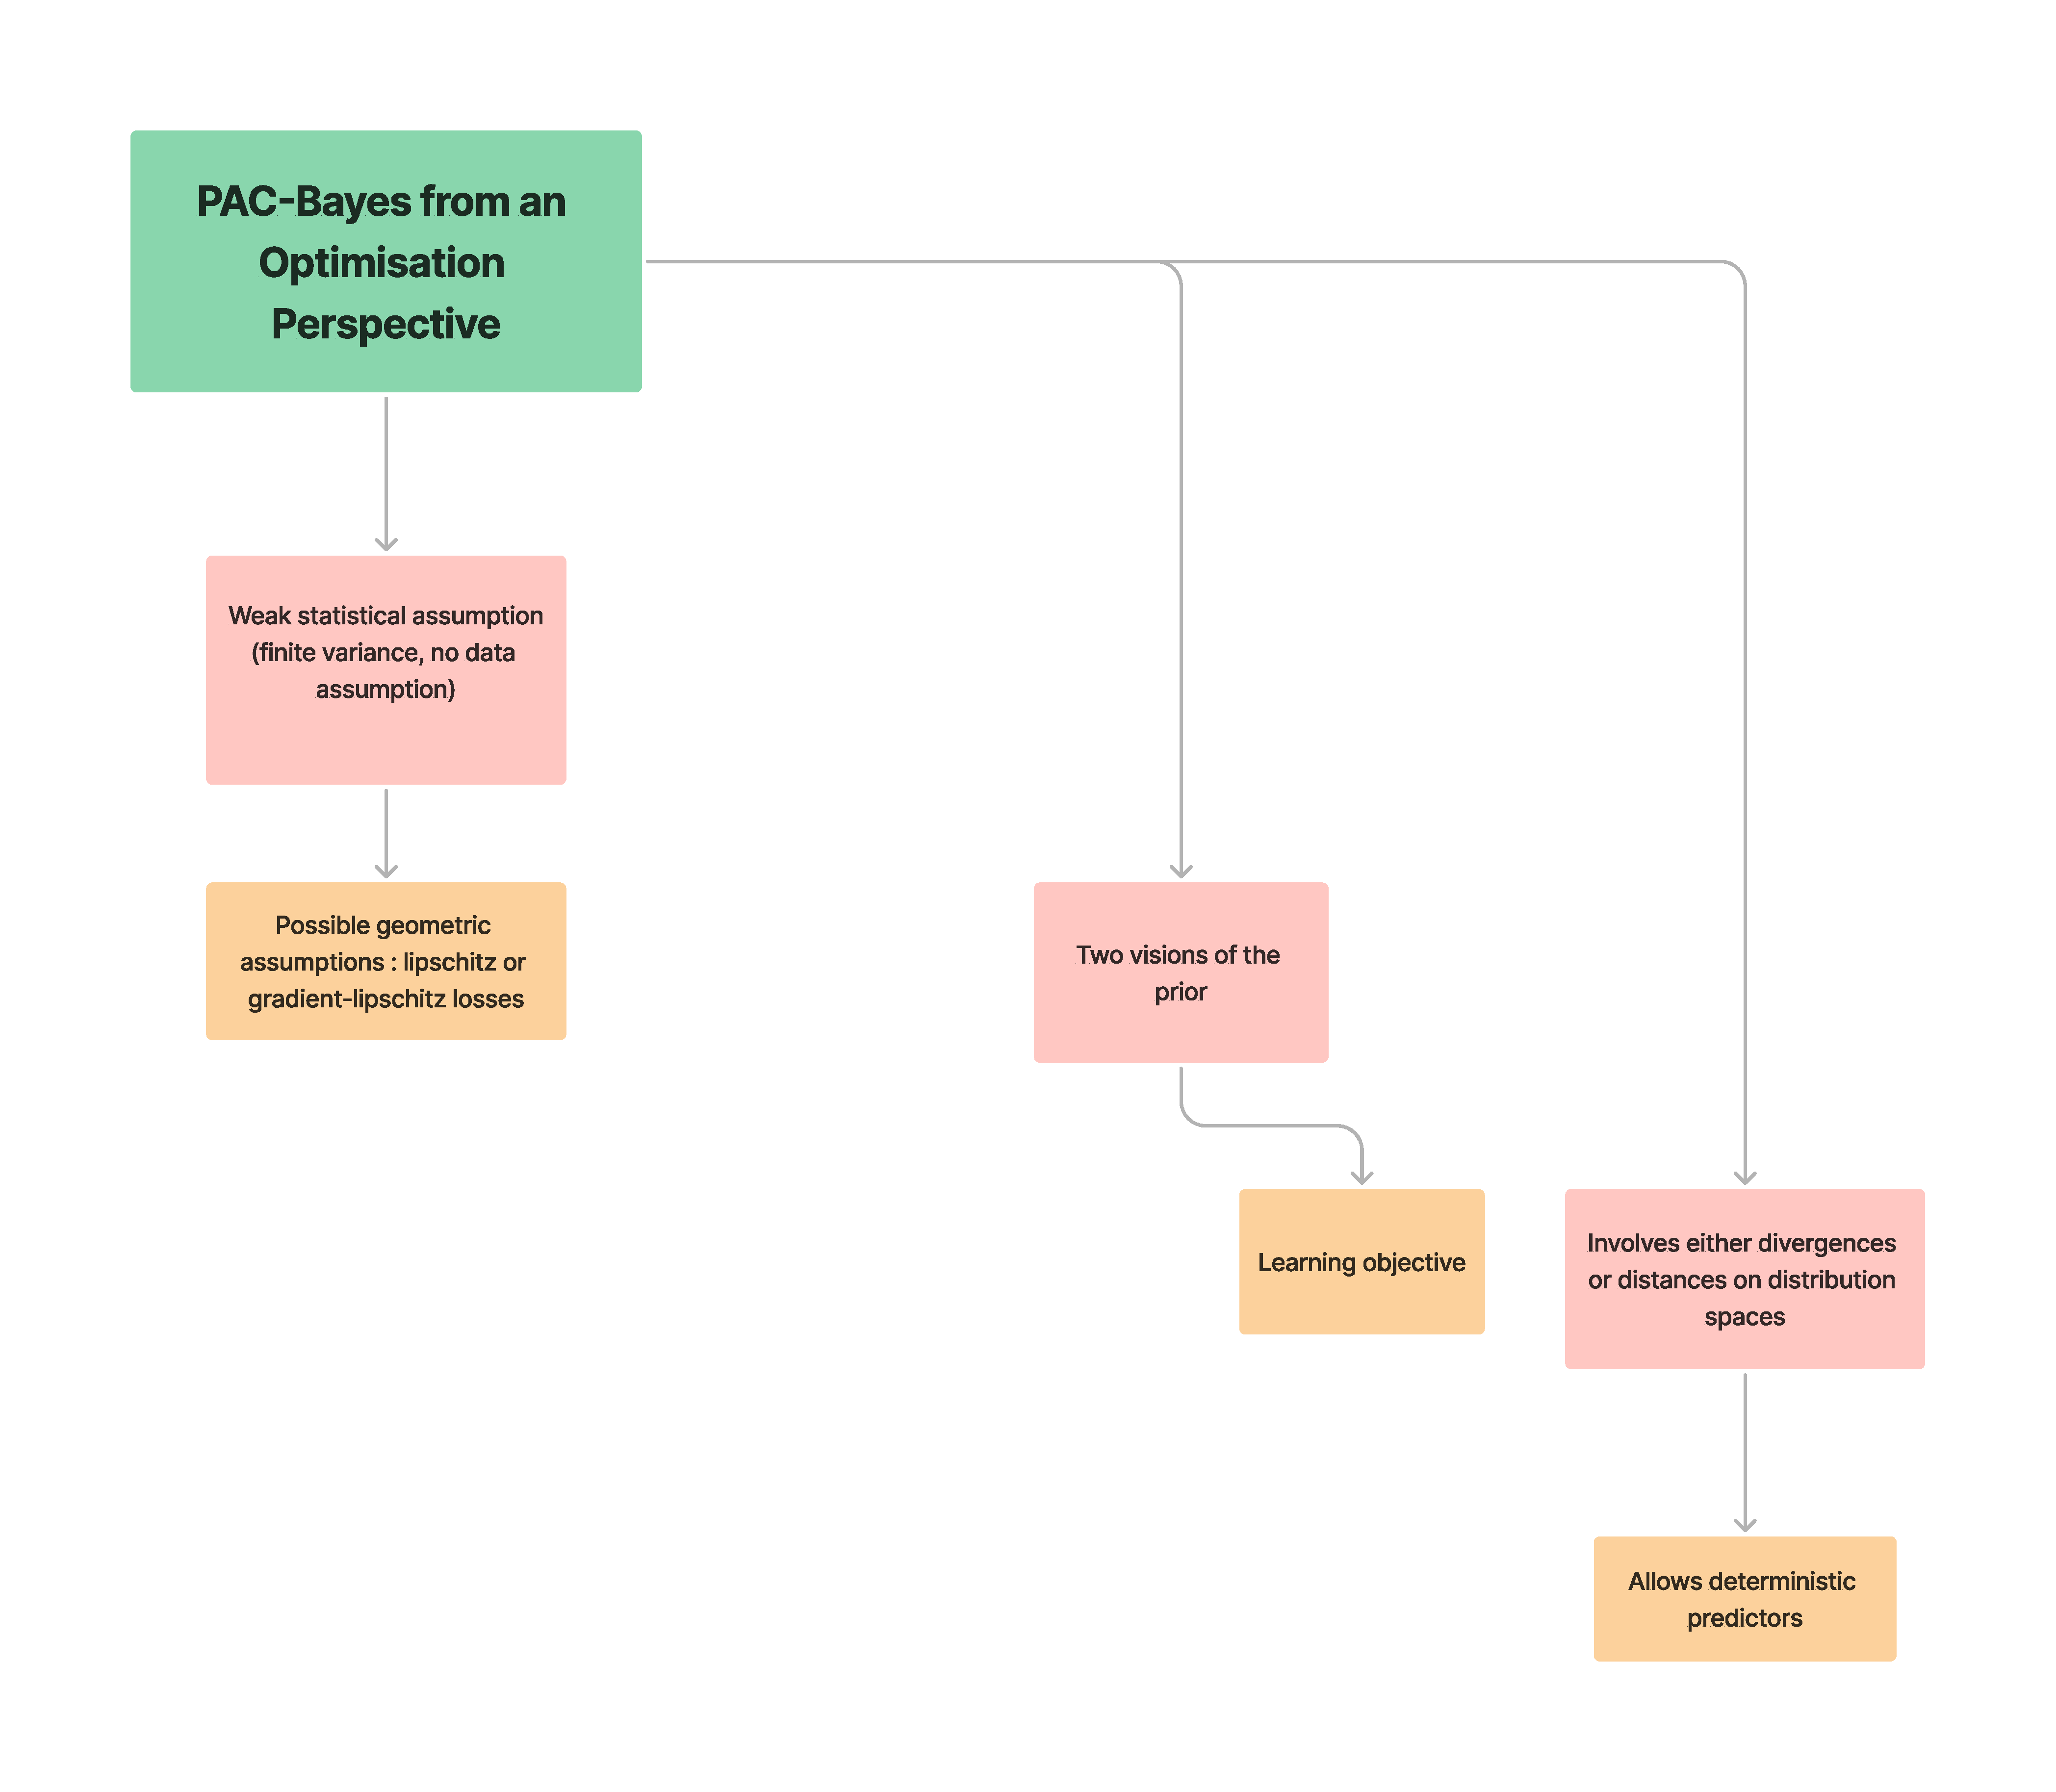
\includegraphics[scale=0.14]{diagram-chap-5.pdf}
    \end{figure}
  \end{xframe}

  \begin{xframe}{Why choosing a Wasserstein distance?}
   \vspace{0.5cm}
   {\Large\bf \green{Two major strength of Wasserstein distances in the optimisation perspective}\\
   \vspace{0.5cm}
   \begin{itemize}
    \item True distances: Dirac priors are allowed
    \item $W_2$ captures a lot of geometric information \eg convergence guarantees for optimisation on measure spaces
   \end{itemize}
   }
   \vspace{0.5cm}
   \uncover<2->{ \bf \Large \orange{Is it possible to obtain WPB bounds with explicit convergence rate?}}
  \end{xframe}

  \begin{xframe}{Presentation of the results}
    \vspace{1.2cm}
    \begin{enumerate}
        \item We obtain WPB bounds for infinite classes of predictors with a classical convergence rate $\mathcal{O}(1/\sqrt{m})$ at the cost of the curse of dimensionality. 

        $\mapsto$ Asymptotic yet interpretable guarantees

        \item We show that it is possible to exploit the geometric convergence guarantees of the \emph{Bures-Wasserstein SGD} to explain its generalisation ability 
    \end{enumerate}
    
\end{xframe}

\begin{xframe}{A WPB bound for compact predictor space}


        \begin{blueblock}{Theorem}
            For any $\delta>0$, assume that $\ell\in[0,1]$ is $K$-Lipschitz wrt to $h$ and that $\mathcal{H}$ is a compact of $\mathbb{R}^d$ bounded in norm by $R$. Let $\P\in \mathcal{P}_1(\mathcal{H})$ a (data-free) prior distribution.
            Then, with probability $1-\delta$ , for any posterior distribution $\Q\in\mathcal{P}_1(\mathcal{H})$:
            \[ |\Delta_S(\Q)| \leq \sqrt{2K(2K+1)\frac{2d\log\left(3\frac{1 +2Rm }{\delta}\right)}{m} \left(W_1(\Q,\P)+\varepsilon_m  \right) + \frac{\log\left( \frac{3m}{\delta} \right)}{m}  }, \]
            with $\varepsilon_m =  \mathcal{O}\left(1 + \sqrt{\frac{d\log(Rm)}{m}}\right)$. 
        \end{blueblock}
    
\end{xframe}

\begin{xframe}{WPB bounds for Gaussian distributions}
    \begin{blueblock}{Theorem}
        Assume that $d\geq 3$, $\mathcal{H}= \mathbb{R}^d$ and that the loss is K-lipschitz. For any $\delta>0, 0\leq \alpha\leq \beta, M\geq 0$, let $\P\in C_{\alpha,\beta,M}$ a (data-free) prior distribution.
        Then, with probability $1-\delta$, for any posterior distribution $\Q\in C_{\alpha,\beta,M}$, the following bound holds.
        
        \textbf{Asymptotic regime} ($d\log(d)< \log(m)$)
        \begin{align*}
        |\Delta_S(\Q)|  \leq\Tilde{\mathcal{O}}\left( \sqrt{2K\frac{d}{m}\left(1 + W_1(\Q,\P)\right)+ (1+K^2\log(m))\frac{\log\left( \frac{m}{\delta} \right)}{m}}   \right).
        \end{align*}
        In all these formulas, $\Tilde{\mathcal{O}}$ hides a polynomial dependency in $(\log(d),\log(m))$.
    \end{blueblock}
\end{xframe}

\begin{xframe}{Remarks}
    \vspace{0.5cm}
    {\bf \Large 
    \begin{itemize}
        \item Bounds for low-data regime ($d\leq m$) and transitory regime ($m>d,\; d\log(d)\geq \log(m)$) are also available in the paper $\rightarrow$ worse dependencies in the dimension
        \item Results for Gaussian $\Q,\P$ and gradient-lipschitz losses available
        \item Trade of statistical assumptions (boundedness) for geometric ones (lipschitz)
        \item For lipschitz losses, Differential Privacy allows replacing $\P$ by a Gibbs posterior (up to negligible terms) 
    \end{itemize}
    }
\end{xframe}




\begin{xframe}{The Bures-Wasserstein SGD }
    \begin{block}{\bf A variational inference algorithm}
        Goal: find $\hat{\Q}$ the best Gaussian approximation of $\Q^*:= \P_{-\frac{\lambda}{2K}\Risk_\S}$ through a sequence $(\hat{\Q}_k)_{k\geq 1}$.
    \end{block}
    \begin{blueblock}{Theorem}
        Assume having a smooth convex loss with a log-strongly convex prior. Under technical assumptions on $\eta,\hat{\Q}_0$, Bures-Wasserstein SGD satisfies for all $k \in \mathbb{N}$,
        $$
        \mathbb{E} W_2^2\left(\hat{\Q}_k, \hat{\Q}\right) \leq \exp (-\alpha k \eta) W_2^2\left(\hat{\Q}_0, \hat{\Q}\right)+\frac{36 d \eta}{\alpha^2} .
        $$
        In particular, $\mathbb{E} W_2^2\left(\hat{\Q}_k, \hat{\Q}\right) \leq \varepsilon^2$ with suitable $\eta,k$.
    \end{blueblock}

\end{xframe}

\begin{xframe}{Exploiting optimisation guarantees for generalisation}
    \begin{block}{\bf Main assumptions}
        \textbf{(A3):} $\mathcal{H}=\mathbb{R}^d$ $\ell$ is twice differentiable, $L$-smooth, convex and  $K$-Lipschitz.
        
       $\P=  \Ncal(0,\Sigma)$ with $\Sigma= \text{diag}(\gamma), 1\geq\gamma>0$. Also $\lambda \leq 2K$ in the definition of $Q^*$.
 
    \end{block}
    \begin{blueblock}{Theorem (informal)}
        Assume \textbf{(A3)}, $d\geq 3$. Let $\beta_m= \mathcal{O}(\frac{1}{\sqrt{m}})$ and fix any $\beta_m<\delta<1$.
        Bures-Wasserstein SGD, with adapted initialisation and parameters $\eta,N$ satisfies, with probability $1-2\delta$:
        
        \noindent \textbf{Asymptotic regime} $(d\log(d)< \log(m))$
        \begin{align*}
        |\Delta_S(\hat{\Q}_N)|  \leq\Tilde{\mathcal{O}}\left( \sqrt{2K\frac{d}{m}\left(1 + W_1(\hat{\Q},\Q^*)\right)+ (1+K^2\log(m)) \frac{\log\left( \frac{m}{\delta} \right)}{m}} \right),
        \end{align*}
        where $\Tilde{\mathcal{O}}$ hides a polynomial dependency in $(\log(d),\log(m))$.
    \end{blueblock}
\end{xframe}

\begin{xframe}{A quick sum up}
    \vspace{1cm}
    {\bf \Large \green{Strength: Wasserstein PAC-Bayes yields generic generalisation bounds with geometric assumption and an interpretable one for the Bures Wasserstein SGD}}
    \\
    \vspace{0.5cm}
    {\bf \Large \red{Drawback: explicit dependency on $d$ $\rightarrow$ vacuous for deep nets }}
    \\
    \vspace{0.5cm}
    {\bf \Large \orange{Can we derive WPB bounds useful for practical optimisation of deep nets? }}


\end{xframe}

\section{Wasserstein PAC-Bayes in Practice: Generalisation-Driven Algorithms for Deterministic Predictors}

\begin{xframe}{Wasserstein PAC-Bayes in Practice}
    \begin{figure}
        \centering
        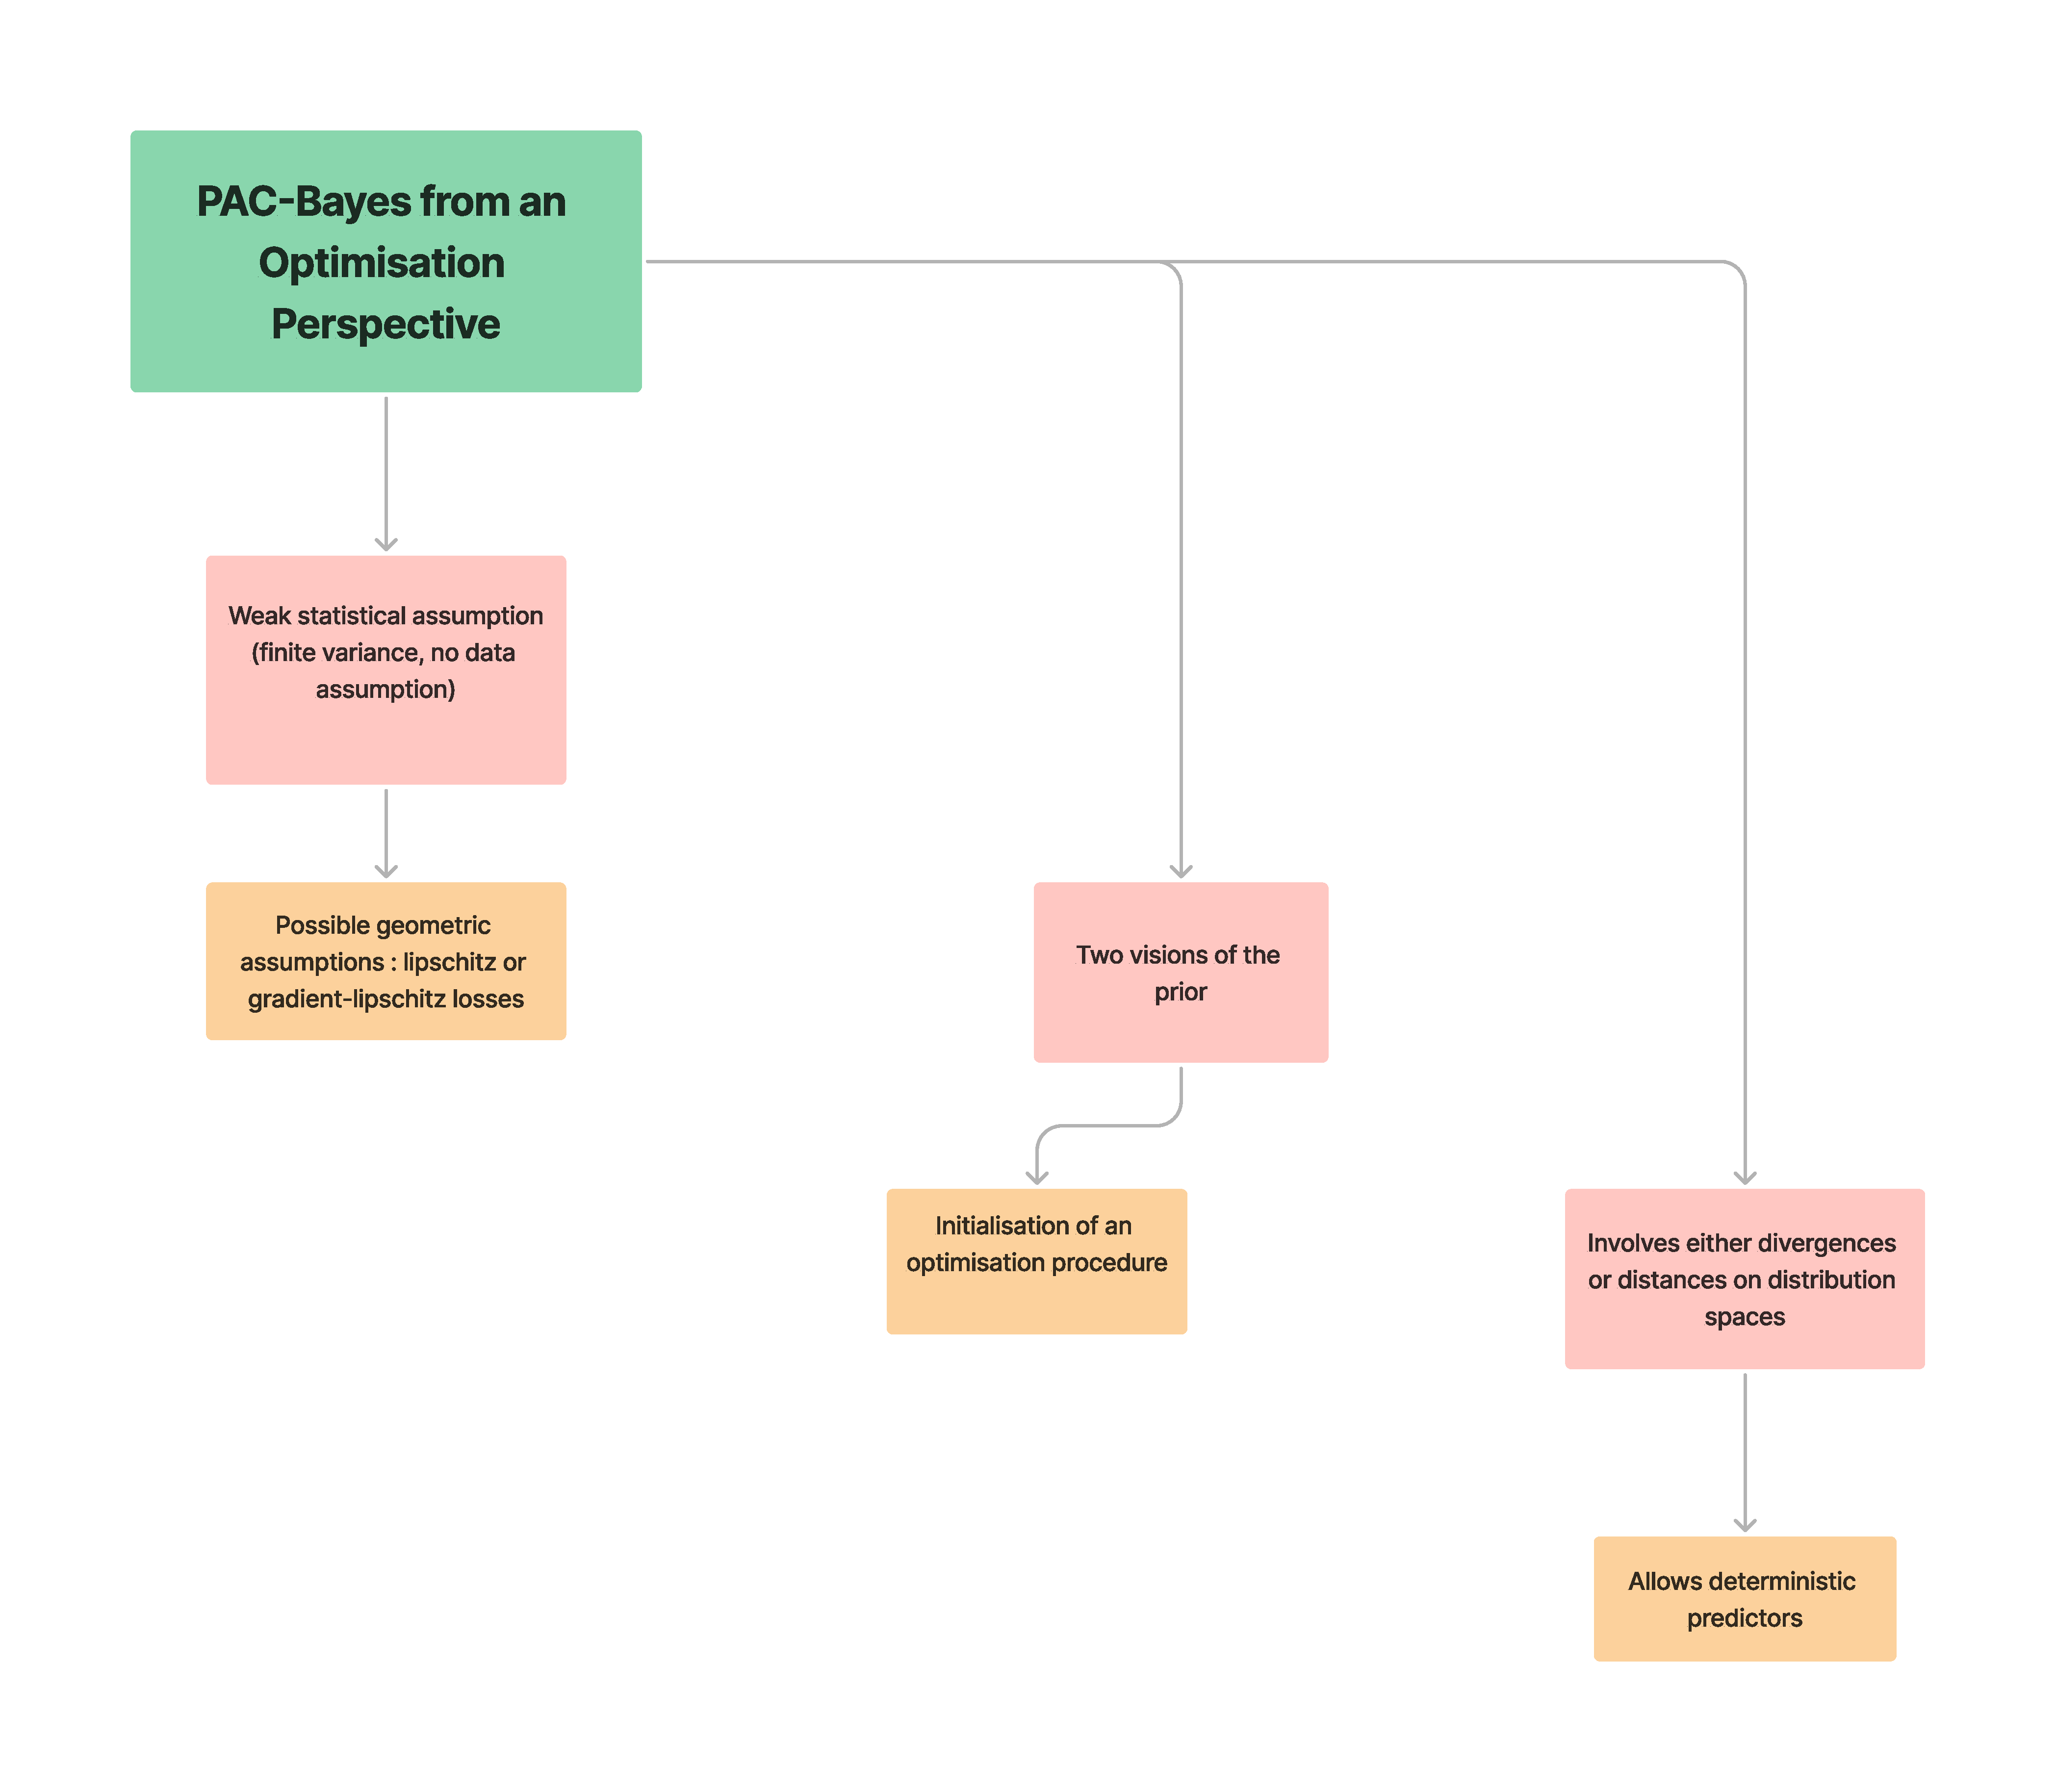
\includegraphics[scale=0.14]{diagram-chap-6.pdf}
    \end{figure}
  \end{xframe}

  \begin{xframe}{WPB bound for batch learning}
    Idea: split $\Sm$ into $L$ parts $\S_1,...,\S_L$ and exploit supermartingale techniques.
    {\bf Assumptions:} 

    \begin{itemize}
        \item $\ell$ is non-negative and $K$-Lipschitz
        \item for any $1\leq i\leq L,\S$, $\EE_{h\sim \P_{i}(.,\S), z\sim \mu}[ \ell(h,z)^2]\leq 1$ 
        \item Prior $\P_{i,\S}$ depend on $\S/\S_i$.
    \end{itemize}
    
    \begin{blueblock}{Theorem}
        For any $\delta\in(0,1]$, with probability at least $1-\delta$ over the sample $\Sm$, the following holds for the distributions $\P_{i,\S}\defeq \P_i(\S,.)$ and for any $\Q\in\Mcal(\Hcal)$: 
        \begin{align*}
        \ \EE_{\h\sim\Q}\left[ \Risk_{\D}(\h) - \hat{\Risk}_{\Sm}(\h) \right] \le \sum_{i=1}^{L} \frac{2|\S_i|K}{m} \W(\Q, \P_{i,\S}) + \sum_{i=1}^{L} \sqrt{\frac{|\S_i|\ln\frac{L}{\delta}}{m^2}}.
        \end{align*}
    \end{blueblock}
\end{xframe}

\begin{xframe}{WPB bound for online learning}
    
    
    {\bf Assumptions:} 
    \begin{itemize}
        \item $\ell$ is non-negative and $L$-Lipschitz
        \item for any $i,\S$, $\EE_{h\sim \P_{i}(.,\S)}\LB \EE_{i-1}[\ell(h,\z_i)^2] \RB \leq 1$ (\emph{bounded order 2 moments for priors})
        \item Sequence of priors $\P_i, i\geq 1$ all past-dependent (online predictive sequence).
    \end{itemize}
    \begin{blueblock}{Theorem}
        For any $\delta\in(0,1]$, with probability at least $1-\delta$ over the sample $\S$, any online predictive sequence (used as priors) $(\P_i)_{i\geq 1}$, we have with probability at least $1-\delta$ over the sample $S\sim\mu$, the following, holding for the data-dependent measures $\P_{i,S}\defeq \P_i(S,.)$ and any posterior sequence $(\Q_i)_{i\geq 1}$:
        
        \begin{align*}
        \frac{1}{m}\sum_{i=1}^m \mathbb{E}_{h_i\sim \Q_{i}} \Big[\mathbb{E}[\ell(h_i,\z_i) \mid \mathcal{F}_{i-1}] - \ell(h_i,\z_i) \Big]  \le \frac{2L}{m}\sum_{i=1}^{m}\W(\Q_{i}, \P_{i,\S}) + \sqrt{\frac{\ln\frac{1}{\delta}}{m}}.
        \end{align*}
    \end{blueblock}
\end{xframe}

\begin{xframe}{New optimisation goals}
    \begin{blueblock}{Batch}
        \begin{align*}
        \operatorname{argmin}_{\h_{\wbf}\in\Hcal} \left\{\hat{\Risk}_{\Sm}(\h_{\wbf}) + \varepsilon\LB\sum_{i=1}^{K} \frac{|\S_i|}{m} \|\wbf-\wbf_i\|_2\RB\right\}.
        \end{align*}
    \end{blueblock}

    \begin{blueblock}{Online}
        \begin{align*}
        \forall i \geq 1, h_i\in  \operatorname{argmin}_{\h_{\wbf}\in\Hcal} \left\{ \loss(\h_{\wbf}, \z_i) + \|\wbf{-}\wbf_{i-1}\| \mid \|\wbf{-}\wbf_{i-1}\| \le 1\right\}.
        \end{align*}
    \end{blueblock}
\end{xframe}


\begin{xframe}{Experiments}
    Classification problem on MNIST solved with linear models and fully connected neural networks.
    \begin{figure}
        \centering
        \includegraphics[scale=0.35]{figures/tables.png}
    \end{figure}
    
\end{xframe}

\section{Conclusion}

\begin{xframe}{Conclusion}
    \vspace{0.5cm}
    \begin{blackblock}{}
        {\bf\Large We challenge the classic perspective on PAC-Bayes.}
    \end{blackblock}
    \vspace{0.5cm}
    \begin{itemize}
        \item \emph{Strong statistical assumptions?} PAC-Bayes bounds hold with finite variance. Sometimes, not even required with (gradient) lispchitz losses. 
        \item \emph{What's perspective for the prior?} We can avoid the Bayesian one: either initialisation point or learning objective $\rightarrow$ novel results to either reduce the impact of the prior or highlight it.
        \item \emph{ PAC-Bayes is useful for stochastic predictors only?} Wasserstein PAC-Bayes shows that it's not $\rightarrow$ deterministic predictors allowed: unveil a novel geometric perspective.
    \end{itemize}
\end{xframe}

\begin{xframe}{Future leads}
    \vspace{0.5cm}
    \begin{redblock}{}
        \red{\bf \Large Many open questions on the interplays of optimisation and generalisation.}
    \end{redblock}
    \vspace{0.5cm}
    \begin{itemize}
        \item Can we relax the finite variance assumption to obtain generalisation bounds?
        \item Can we further exploit flat minima to understand generalisation?
        \item Can we reach Wasserstein PAC-Bayes bound as simple and efficient than a KL one? 
        \item Investigating the links between Online Learning and Wasserstein PAC-Bayes (directly using the 2 Wasserstein)?
    \end{itemize}

\end{xframe}

\begin{xframe}{}
    \vspace{4cm}

        \centering{\bf \LARGE Thank you for your attention !}


\end{xframe}




%%%%%%%%%%%%%%%%%%%%%%%%%%%%%%%%%%%%%%%%%%%%%%%%%%%%%%%%%%%%%%%%%%%%%%%%%%%%%%%


%%%%%%%%%%%%%%%%%%%%%%%%%%%%%%%%%%%%%%%%%%%%%%%%%%%%%%%%%%%%%%%%%%%%%%%%%%%%%%%



%%%%%%%%%%%%%%%%%%%%%%%%%%%%%%%%%%%%%%%%%%%%%%%%%%%%%%%%%%%%%%%%%%%%%%%%%%%%%%%

\appendix

\begin{frame}[t,noframenumbering,allowframebreaks]
  \frametitle{References}
  \printbibliography[title={References}]
 \end{frame}

\begin{xtitle}

\vspace{2.0cm}
{\bf Thank you for your attention!}\\

\end{xtitle}

%%%%%%%%%%%%%%%%%%%%%%%%%%%%%%%%%%%%%%%%%%%%%%%%%%%%%%%%%%%%%%%%%%%%%%%%%%%%%%%
 
\end{document}